% =====================================================
% TP final FasoPay - Groupe 07
% YAMEOGO Joseph, ZONGO Abdrafith
% Compilation : pdflatex (F5 dans TeXstudio), DEUX FOIS pour le sommaire
% =====================================================
\documentclass[11pt,a4paper]{article}

% ---------- Langue, police, accents ----------
\usepackage[T1]{fontenc}
\usepackage[utf8]{inputenc}
\usepackage{lmodern}
\usepackage[french]{babel}
\frenchsetup{AutoSpacePunctuation=false}   % pas d'espace ajoutée dans 08:25 ou w:1

% ---------- Mise en page ----------
\usepackage[a4paper,margin=2.0cm]{geometry}
\usepackage{graphicx}
\graphicspath{{../images/}}   % les images sont dans le dossier images/, à côté de rapport/
\usepackage{float}
\usepackage{caption}
\usepackage{booktabs}
\usepackage{tabularx}
\usepackage{longtable}
\usepackage{array}
\usepackage{enumitem}
\setlist{itemsep=2pt,topsep=4pt}
\usepackage[table]{xcolor}
\usepackage{fancyhdr}

% ---------- Couleurs ----------
\definecolor{bleufaso}{RGB}{43,108,176}
\definecolor{grisfond}{RGB}{246,248,250}
\definecolor{griscode}{RGB}{90,90,90}

% ---------- Code (mongosh, PowerShell) ----------
\usepackage{listings}
\lstset{
	basicstyle=\ttfamily\small,
	backgroundcolor=\color{grisfond},
	frame=single, rulecolor=\color{black!15},
	breaklines=true, columns=fullflexible,
	keepspaces=true, showstringspaces=false,
	commentstyle=\color{griscode}\itshape,
	literate={é}{{\'e}}1 {è}{{\`e}}1 {ê}{{\^e}}1 {à}{{\`a}}1 {â}{{\^a}}1
	{ù}{{\`u}}1 {û}{{\^u}}1 {ô}{{\^o}}1 {î}{{\^i}}1 {ç}{{\c c}}1
	{É}{{\'E}}1 {È}{{\`E}}1 {À}{{\`A}}1 {Ç}{{\c C}}1
	{«}{{\guillemotleft}}1 {»}{{\guillemotright}}1 {œ}{{\oe}}1 {ï}{{\"i}}1
	{×}{{$\times$}}1 {·}{{$\cdot$}}1 {→}{{$\rightarrow$}}1 {−}{{-}}1 {≥}{{$\geq$}}1 {°}{{\textdegree}}1 {’}{{'}}1 {–}{{--}}1 {≈}{{$\approx$}}1 {÷}{{$\div$}}1
}


% ---------- Ajouts : tableaux, caractères spéciaux, paragraphes ----------
\usepackage{amsmath}
\usepackage{needspace}   % garde un titre avec la suite
\usepackage{calc}        % largeurs de colonnes des tableaux des annexes
\usepackage{textcomp}
\newcolumntype{L}{>{\raggedright\arraybackslash}X}
\newcolumntype{P}[1]{>{\raggedright\arraybackslash}p{#1}}   % colonne de largeur fixe alignée à gauche   % colonne X alignée à gauche
\providecommand{\tightlist}{\setlength{\itemsep}{0pt}\setlength{\parskip}{0pt}}
\DeclareUnicodeCharacter{2212}{\ensuremath{-}}       % −
\DeclareUnicodeCharacter{2194}{\ensuremath{\leftrightarrow}} % ↔
\DeclareUnicodeCharacter{2192}{\ensuremath{\rightarrow}} % →
\DeclareUnicodeCharacter{2265}{\ensuremath{\geq}}    % ≥
\DeclareUnicodeCharacter{2264}{\ensuremath{\leq}}    % ≤
\DeclareUnicodeCharacter{2248}{\ensuremath{\approx}} % ≈
\DeclareUnicodeCharacter{2260}{\ensuremath{\neq}}    % ≠
\DeclareUnicodeCharacter{2076}{\textsuperscript{6}}  % ⁶
\DeclareUnicodeCharacter{2079}{\textsuperscript{9}}  % ⁹
\setlength{\parindent}{0pt}
\setlength{\emergencystretch}{3em}   % évite les lignes qui débordent à cause du code
\setlength{\parskip}{4pt plus 1pt}
\renewcommand{\arraystretch}{1.15}
\captionsetup{font=small,labelfont=bf,justification=centering}
% \code{...} : du code dans le texte (les _ et $ s'écrivent tels quels)
\newcommand{\code}[1]{\texttt{\detokenize{#1}}}
% Encadré « ce qu'il faut retenir »
\newcommand{\retenir}[1]{\par\smallskip\noindent\colorbox{grisfond}{\parbox{\dimexpr\linewidth-2\fboxsep}{\small\textbf{À retenir.} #1}}\par\smallskip}

% ---------- Liens cliquables (toujours en dernier) ----------
\usepackage[hidelinks]{hyperref}
% \gl{n} : petit numéro cliquable qui renvoie au mot n du lexique (annexe G)
\newcommand{\gl}[1]{\textsuperscript{\hyperlink{lex#1}{#1}}}

% ---------- En-tête et pied de page ----------
\pagestyle{fancy}
\fancyhf{}
\fancyhead[L]{\small TP final FasoPay · Groupe 07}
\fancyhead[R]{\small\leftmark}
\fancyfoot[C]{\thepage}
\renewcommand{\headrulewidth}{0.4pt}
\setlength{\headheight}{14pt}

% Petit raccourci pour citer une preuve : \preuve{05-failover.txt}
\newcommand{\preuve}[1]{\texttt{preuves/#1}}


\begin{document}
	
	% =====================================================
	% PAGE DE TITRE
	% =====================================================
	\begin{titlepage}
		\centering
		\begin{minipage}[c]{0.45\textwidth}
			\raggedright
			
\includegraphics[height=2.6cm]{University-Joseph-Ki-Zerbo.jpg}
		\end{minipage}
		\hfill
		\begin{minipage}[c]{0.45\textwidth}
			\raggedleft
			
\includegraphics[height=2.6cm]{logo_IFOAD.jpeg}
		\end{minipage}
		
		\vspace{1.2cm}
		{\large Université Joseph KI-ZERBO (UJKZ)\par}
		\vspace{0.1cm}
		{\large Institut de Formation Ouverte et à Distance (IFOAD)\par}
		\vspace{0.3cm}
		{\large Master 2 Data Science\par}
		\vspace{0.2cm}
		{\normalsize UE Bases de données NoSQL\par}
		
		\vspace{2cm}
		{\color{bleufaso}\rule{\linewidth}{1.2pt}\par}
		\vspace{0.5cm}
		{\Huge\bfseries TP final FasoPay\par}
		\vspace{0.4cm}
		{\Large Audit, conception et démonstration\\[2pt]
			d'un portefeuille de paiement mobile sur MongoDB\par}
		\vspace{0.5cm}
		{\color{bleufaso}\rule{\linewidth}{1.2pt}\par}
		
		\vspace{2cm}
		{\Large\bfseries Groupe 07\par}
		\vspace{0.4cm}
		{\large YAMEOGO Joseph\par}
		\vspace{0.1cm}
		{\large ZONGO Abdrafith\par}
		
		\vfill
		{\large Enseignant : M. Gael BARRY\par}
		\vspace{0.4cm}
		{\small Dépôt Git : \url{https://github.com/Abdrafith-ZONGO/TP_Faso_FasoPay_G7}\par}
		\vspace{0.6cm}
		{\normalsize Année universitaire 2026-2027 \quad·\quad Novembre 2026\par}
	\end{titlepage}
	
	% =====================================================
	% SOMMAIRE
	% =====================================================
	\setcounter{tocdepth}{1}
	\tableofcontents
	\newpage
	
	% =====================================================
	% 1. CONTEXTE ET PROBLÉMATIQUE
	% =====================================================
	\section{Contexte et problématique}
	
	FasoPay, la filiale de paiement mobile de Faso Hub, vise 3 millions de wallets\gl{76} et 400 millions de transactions par an à 18 mois, avec un pic de 1 200 transactions par seconde, une disponibilité de 99,95 \% et \textbf{aucune perte d'argent acceptable} (RPO\gl{60} de 0). Son CTO\gl{20} nous confie quatre demandes, qui structurent ce rapport :
	
	\begin{center}\small
		\begin{tabularx}{\linewidth}{@{}P{5.6cm}LL@{}}
			\toprule
			\textbf{Demande du CTO} & \textbf{Notre réponse} & \textbf{Où} \\
			\midrule
			(1) un modèle de données solide & ledger en partie double, validateurs qui rejettent, solde traité comme un cache & Parties 0 et 1 \\
			(2) retrouver les soldes incohérents & 6 wallets trouvés et chiffrés, plus le découpage, le CA et les rejeux & Partie 2 \\
			(3) des virements qui ne doublent ni ne se perdent & \code{transfer()} : idempotence, abort prouvé, concurrence, pannes réelles & Parties 3, 4, 5 \\
			(4) une architecture sans « usine à gaz » & cible PME chiffrée, chaque composant écarté avec son seuil de retour & Parties 6, 7 \\
			\bottomrule
		\end{tabularx}
	\end{center}
	
	\textbf{Notre principe de travail.} Nous ne prétendons rien que nous n'ayons mesuré nous-mêmes. Chaque chiffre de ce rapport renvoie à un fichier de \code{preuves/} (commande exacte, date \code{date -u}, sortie brute), produit par une commande de l'annexe B. Quand une mesure contredit notre architecture, nous la montrons au lieu de la cacher (Partie 0).
	
	\subsection*{Notre jeu de données}
	2 000 clients, 150 marchands, 60 000 transactions sur 181 jours, du 31 décembre 2025 au 30 juin 2026 (heures UTC). Notre vérification D3, écrite par nous, retrouve chaque chiffre du \code{fingerprint.json}\gl{26} (\preuve{00-fingerprint.txt}) :
	
	\begin{center}\small
		\begin{tabular}{@{}lrr@{}}
			\toprule
			\textbf{Grandeur} & \textbf{Attendu} & \textbf{Obtenu} \\
			\midrule
			customers / wallets / merchants & 2 000 / 2 000 / 150 & 2 000 / 2 000 / 150 \\
			transactions / ledger\_entries & 60 000 / 141 939 & 60 000 / 141 939 \\
			somme des \code{amount} (toutes / \code{COMPLETED}) & 2 018 172 375 / 1 946 303 325 & identiques \\
			somme des \code{balance} des wallets & 832 251 836 & 832 251 836 \\
			empreintes SHA-256 des 5 fichiers NDJSON & 5 & 5 conformes \\
			\bottomrule
		\end{tabular}
	\end{center}
	
	Les types ont été contrôlés après l'import : montants en \code{int}, dates en \code{date}, seul \code{feePct} en \code{double} (\preuve{00-types.txt}). Les collections de traitement \code{outbox}\gl{44} et \code{fraud_alerts} ont été créées vides (D4).
	
	\subsection*{Notre environnement}
	Windows, Docker 29.8.0, MongoDB 8.0.34 (image \code{mongo:8.0}) et mongosh 2.14.0, avec environ 8,17 Go de mémoire visibles par Docker. Nous avons monté nous-mêmes quatre environnements, tous décrits commande par commande en annexe B : le serveur du TP \code{mongo-rs1} (Replica Set\gl{54} \code{rs0} à un nœud, Parties 0 à 4), le Replica Set \code{rs-fasopay} à trois nœuds (Partie 5), un cluster shardé à trois shards\gl{63} (Partie 6) et un serveur de test avec authentification (Partie 7). La contribution de chaque membre est détaillée en annexe F.
	
	\textbf{Pourquoi un Replica Set, même à un seul nœud ?} Les transactions multi-documents\gl{69}, indispensables à un virement (Partie 4), s'appuient sur l'oplog\gl{42}, le journal des opérations que tient un Replica Set. Un serveur MongoDB isolé les refuse. Le mode Replica Set est donc obligatoire dès la Partie 0, même avec un seul membre ; à un nœud, la majorité vaut 1 et \code{w: "majority"}\gl{79} équivaut à \code{w: 1}, ce qui nous a conduits à rejouer nos tests sur trois nœuds (Partie 5). État vérifié : \code{set: rs0}, \code{myState: 1} (PRIMARY), un membre (\preuve{00-rs-status-1-noeud.txt}).
	
	% =====================================================
	% 2. PARTIE 0 : DIMENSIONNEMENT
	% =====================================================
	\section{Partie 0 · Dimensionnement}
	
	Avant de choisir une architecture, il faut savoir quelle quantité de données FasoPay devra stocker et traiter dans 18 mois. Nous ne pouvons pas mesurer directement 400 millions de transactions : nous mesurons donc la taille réelle de nos documents sur notre jeu de 60 000 transactions, puis nous la multiplions jusqu'à la cible. Ces chiffres décident ensuite de tout le reste : combien de serveurs, combien de mémoire, et s'il faut répartir les données sur plusieurs machines (le sharding).
	
	Nous avons mesuré nos documents avec \code{$bsonSize} sur toute la collection, et la taille des données et des index\gl{30} avec \code{$collStats} (\preuve{00-dimensionnement.txt} ; feuille complète en annexe A). Une transaction pèse 253 octets, une ligne de ledger\gl{34} 130, et une transaction métier écrit 2,37 lignes de ledger : 561 octets par transaction métier.
	
	De ces mesures, nous déduisons les besoins de FasoPay à 18 mois :
	
	\begin{center}\small
		\begin{tabularx}{\linewidth}{@{}lLr@{}}
			\toprule
			\textbf{Grandeur à 18 mois} & \textbf{Calcul} & \textbf{Résultat} \\
			\midrule
			Données par an & $400\,\text{M} \times 561{,}02$ octets & 224,4 Go \\
			Avec index & facteur d'index mesuré $\times 1{,}37$ (après les index de la Partie 3) & 307,9 Go \\
			Écritures au pic & $1\,200$ tx/s $\times$ 6 documents (ADR-001) & 7 200 documents/s \\
			Working set & 30 jours de transactions (18,4 Go) + leurs index (6,9 Go) + 3 M wallets et leur index (0,6 Go) & \textbf{25,9 Go} \\
			RAM par nœud & cache $\approx 50\,\% \times (\text{RAM} - 1\,\text{Go}) \geq 25{,}9$ Go, donc RAM $\geq 52{,}8$ Go & \textbf{64 Go} \\
			Disque & 198,5 Go par an après compression (0,51 mesurée), sur 700 Go utilisables (2 × 1 To en RAID 1) & 3,5 ans \\
			Facteur de pic & pic $\div$ moyenne $= 1\,200 \div 12{,}7$ & $\times 95$ \\
			\bottomrule
		\end{tabularx}
	\end{center}
	
	Le facteur de pic de 95 est la leçon de cette feuille : \textbf{nous dimensionnons sur le pic, pas sur la moyenne}. Ces chiffres pointent vers une architecture proportionnée : un seul Replica Set, sans sharding, sans Spark, sans Redis et sans Kafka au démarrage. Chaque composant écarté a un seuil de retour chiffré (annexe A, section 3), par exemple le sharding à 490 M transactions par an sur des nœuds de 64 Go.
	
	\textbf{Deux chiffres qui contredisent notre verdict, et ce que nous en faisons.}
	\begin{itemize}
		\item \textbf{La taille des index.} Nos index pèsent 27 octets par entrée, parce qu'un index de 60 000 documents reste compact. À grande échelle, on compte plutôt 40 à 60 octets (chapitre 11). À 60 octets, le working set\gl{78} monterait à 34,3 Go et \textbf{64 Go ne suffiraient plus}. Nous gardons 64 Go, avec un seuil de surveillance : au-delà de 45 octets par entrée, nous passons à des nœuds de 128 Go (une montée en gamme, pas un sharding).
		\item \textbf{Le débit d'écriture.} Sur notre ordinateur portable, \code{transfer()} atteint 330 virements/s avec 4 clients (Partie 4). Pour que le pic de 1 200 n'occupe que la moitié du primary\gl{49}, il en faudrait 2 400. La mesure ne vaut pas pour un serveur, mais elle nous impose une décision : \textbf{un test de charge sur le matériel cible avant la mise en production}.
	\end{itemize}
	
	\retenir{un Replica Set de nœuds de 64 Go tient la cible à 18 mois en volume et en mémoire ; le débit du primary au pic reste à prouver sur le matériel cible, et nous le disons.}
	
	% =====================================================
	% 3. PARTIE 1 : MODÉLISATION
	% =====================================================
	\section{Partie 1 · Modélisation (ADR-001)}
	
	Un modèle de données décide de ce que la base accepte, de la façon dont les informations sont rangées et de ce que coûte chaque lecture. Pour FasoPay, il doit surtout protéger l'argent : refuser un montant faux, garder la trace de chaque mouvement et permettre de retrouver un solde contesté. Nous présentons d'abord les règles que la base impose à chaque document, puis, relation par relation, notre choix entre l'embedding\gl{22}, qui range une information dans le document qui l'utilise, et le referencing\gl{53}, qui la range dans une autre collection, et enfin le grand livre qui garde la trace de l'argent.
	
	\subsection{Un schéma qui rejette ce qui est faux}
	\sloppy Six collections portent un validateur\gl{75} \code{$jsonSchema} en \code{validationLevel: "strict"} et \code{validationAction: "error"} : \code{customers}, \code{wallets}, \code{merchants}, \code{transactions}, \code{ledger_entries} et \code{outbox}. Les montants sont des entiers (\code{int} ou \code{long}) : un franc CFA ne se divise pas, et un \code{double} introduirait des arrondis. Le validateur de \code{ledger_entries} utilise \code{oneOf} pour accepter les deux formes de ligne : une jambe de wallet (\code{walletId} et \code{balanceAfter}\gl{5} obligatoires) ou une jambe hors wallet (\code{walletId: null} et un compte \code{FEES}, \code{FLOAT}, \code{BILLER} ou \code{MERCHANT:M…}).
	
	Preuve (\preuve{01-validator-rejet.txt}) : nos 206 089 documents passent tous (0 invalide), et un document invalide est \textbf{rejeté dans chaque collection} avec le code 121 et son détail \code{errInfo} (par exemple \code{balance: 12.5} ou \code{kycLevel: 'trois'}).
	
	\subsection{Embedding ou referencing : relation par relation}
	\begin{center}\small
		\begin{tabularx}{\linewidth}{@{}P{3.6cm}P{2.6cm}L@{}}
			\toprule
			\textbf{Relation} & \textbf{Choix} & \textbf{Justification mesurée} \\
			\midrule
			client ↔ wallet & referencing & 1 wallet par client ; le wallet change à chaque virement, le client presque jamais \\
			wallet ↔ transactions & referencing & une transaction concerne deux wallets ; jusqu'à 319 transactions par wallet \\
			transaction ↔ ledger & referencing (collection séparée) & 2 à 6 lignes par transaction, relues par wallet (historique) et pas seulement par transaction \\
			transaction ↔ tentatives & embedding & les rejeux se lisent avec leur transaction ; seules 21 en ont \\
			ledger ↔ solde & copie (\code{balanceAfter}) & l'historique d'un wallet se lit sans recalcul (Computed pattern) \\
			\bottomrule
		\end{tabularx}
	\end{center}
	
	\subsection{Quatre access patterns, par fréquence × criticité}
	\begin{center}\small
		\begin{tabularx}{\linewidth}{@{}lLlll@{}}
			\toprule
			& \textbf{Access pattern} & \textbf{Au pic} & \textbf{Latence cible} & \textbf{Cohérence} \\
			\midrule
			AP1 & exécuter un virement (avec la clé d'idempotence) & 1 200/s & p95 < 300 ms & forte \\
			AP2 & lire son solde (USSD, application) & milliers/s & p95 < 100 ms & forte (primary) \\
			AP3 & historique d'un wallet, trié, paginé & centaines/s & p95 < 150 ms & retard toléré \\
			AP4 & contrôles de nuit : rapprochement (E1), plafond (E2) & 1 par nuit & minutes & photo figée \\
			\bottomrule
		\end{tabularx}
	\end{center}
	AP1 est le plus critique (c'est de l'argent, au pic), AP2 le plus fréquent. AP4 est rare, mais c'est lui qui détecte les écarts dont se plaint le CTO.
	
	\subsection{L'anti-pattern évité : le ledger embarqué dans le wallet}
	Mettre les lignes de ledger dans un tableau du wallet semble naturel. Mesuré sur nos données : 35,94 lignes par wallet en moyenne et 390 au maximum, soit 4 831 octets en moyenne et 52 346 au maximum, après six mois seulement. Le wallet, document le plus modifié de la base, grossirait à chaque virement et serait réécrit en entier, jusqu'à la limite de 16 Mo (environ 125 000 lignes). Nous gardons donc le ledger séparé, relié par \code{walletId}.
	
	\subsection{Un grand livre en partie double}
	Notre modèle applique les règles d'un grand livre, toutes vérifiées sur nos données : \textbf{montants entiers} en FCFA\gl{25} ; \textbf{partie double\gl{46}} (débits = crédits = 1 955 479 314 FCFA, 0 transaction déséquilibrée sur 56 484) ; \textbf{ajout seul} (les 280 transactions \code{REVERSED} gardent leurs lignes d'origine et reçoivent des lignes inverses, \preuve{01-mesures-modelisation.txt}) ; \textbf{le solde est un cache\gl{66}} du ledger, qui doit changer dans la même transaction que lui, sinon il diverge (ce que mesure E1) ; \textbf{idempotence\gl{29}} par un index unique\gl{32} (Partie 3).
	
	\textbf{ADR-001\gl{3} (décision).} Un virement écrit \textbf{6 documents dans une seule transaction multi-documents} : la transaction, deux lignes de ledger, deux soldes et un événement \code{outbox}. Rejetés : la transaction seule (aucun solde auditable), le solde recalculé à chaque lecture (35,94 lignes en moyenne, toujours plus), le solde sans ledger (aucune trace pour un solde contesté). Coût accepté : 7 200 écritures/s au pic. ADR complet dans \code{adr/ADR-001.md}.
	
	\retenir{la base refuse désormais les documents faux, chaque mouvement d'argent est écrit deux fois dans un journal qui ne s'efface jamais, et un virement écrit ses 6 documents ensemble ou pas du tout.}
	
	% =====================================================
	% 4. PARTIE 2 : ENQUÊTE
	% =====================================================
	\section{Partie 2 · Enquête : E1, E2, E3, E4}
	
	Le CTO nous pose quatre questions sur des problèmes réels : des soldes contestés, des clients qui contourneraient leur plafond, la concentration du chiffre d'affaires et des paiements en double. Pour y répondre, nous interrogeons directement nos données, et chaque réponse est chiffrée et vérifiable.
	
	Chaque pipeline\gl{4} commence par un \code{$match} qui réduit les documents le plus tôt possible ; l'ordre des étapes est commenté dans \code{code/02-enquete.js}. Toutes les réponses se rattachent au \code{fingerprint.json} (\preuve{02-enquete.txt}).
	
	\subsection{E1 : les soldes qui ne collent pas au ledger}
	La finance dit que « le ledger ne colle pas aux soldes ». Si c'est vrai, le solde stocké dans certains wallets doit être différent du total de leurs mouvements dans le ledger : c'est ce que nous cherchons.
	
	Pour chaque wallet, nous additionnons ses lignes de ledger (crédit +, débit −) et comparons à \code{wallets.balance}. Le \code{$match} écarte d'abord les 70 054 lignes sans wallet, et le \code{$group} précède le \code{$lookup}\gl{35} : 2 000 jointures au lieu de 71 885.
	
	\begin{center}\small
		\begin{tabular}{@{}lrrrr@{}}
			\toprule
			\textbf{Wallet} & \textbf{Solde stocké} & \textbf{Solde du ledger} & \textbf{Écart} & \textbf{Lignes} \\
			\midrule
			W001124 & 249 025 & 278 025 & −29 000 & 7 \\
			W001372 & 557 152 & 585 152 & −28 000 & 33 \\
			W000967 & 389 447 & 415 447 & −26 000 & 28 \\
			W001796 & 949 293 & 960 793 & −11 500 & 49 \\
			W000668 & 478 654 & 487 654 & −9 000 & 31 \\
			W000769 & 75 692 & 41 192 & +34 500 & 86 \\
			\bottomrule
		\end{tabular}
	\end{center}
	
	\textbf{6 wallets sur 2 000 sont incohérents.} Les écarts se compensent en partie : l'écart net (−69 000 FCFA) sous-estime le problème, nous retenons l'\textbf{écart absolu de 138 000 FCFA}. \textbf{Rattachement :} le ledger signé des wallets totalise 832 320 836, les soldes 832 251 836 (fingerprint) ; la différence, 69 000, est exactement l'écart net : rien d'autre ne diverge. Pour ces 6 wallets, le dernier \code{balanceAfter} du ledger égale la somme du ledger : \textbf{c'est le solde stocké qui a divergé, pas le ledger}. Le correctif passe par des écritures d'ajustement dans le ledger, pas par une modification directe du solde.
	
	\subsection{E2 : les clients qui découpent leurs transferts}
	La conformité soupçonne des clients de découper leurs transferts en plusieurs montants juste sous leur plafond journalier. Il faut d'abord définir ce qu'est un découpage, puis chercher les wallets qui correspondent.
	
	\textbf{Notre critère, explicite :} un wallet est suspect un jour donné s'il émet au moins 3 sorties \code{COMPLETED} (\code{P2P} ou \code{CASH_OUT}) comprises chacune entre 90 \% et 100 \% de son plafond \code{dailyLimit}. Les sorties vers une personne ou en espèces sont les transferts ; la bande 90--100 \% décrit un montant choisi pour rester juste sous la limite ; le seuil de 3 évite de signaler un cas isolé.
	
	\textbf{Résultat : 5 wallets}, 23 couples wallet-jour, 121 transactions. Le critère est solide : aucune sortie ne dépasse le plafond à elle seule (0 sur 46 495), aucun autre wallet n'a de transaction dans la bande, et avec un seuil de 50 \% ou 70 \% nous retrouvons les mêmes 5 wallets. \textbf{Le contournement est un problème de cumul, pas de montant.}
	
	\textbf{Cas détaillé : W000758, le 30 janvier 2026} (plafond 200 000 FCFA). Sept sorties en moins de 3 heures, espacées de 21 à 41 minutes :
	\begin{center}\small
		\begin{tabular}{@{}lllr@{}}
			\toprule
			\textbf{Heure (UTC)} & \textbf{Type} & \textbf{Destinataire} & \textbf{Montant (FCFA)} \\
			\midrule
			08:25 & CASH\_OUT & --- & 191 375 \\
			08:54 & P2P & W000951 & 186 050 \\
			09:20 & CASH\_OUT & --- & 189 575 \\
			09:41 & P2P & W001312 & 181 850 \\
			10:17 & P2P & W001312 & 191 975 \\
			10:40 & P2P & W000951 & 191 475 \\
			11:21 & CASH\_OUT & --- & 188 025 \\
			\midrule
			\multicolumn{3}{@{}l}{\textbf{Total de la matinée}} & \textbf{1 320 325} \\
			\bottomrule
		\end{tabular}
	\end{center}
	Soit 6,6 fois le plafond en une matinée, vers deux bénéficiaires seulement. Un indice n'est pas une preuve de fraude : ces 5 wallets sont la liste de départ de la conformité, et le contrôle cumulatif doit devenir automatique (alerte dans \code{fraud_alerts}, Partie 7).
	
	\subsection{E3 : les marchands qui concentrent le chiffre d'affaires}
	Le CTO veut savoir si quelques marchands font l'essentiel du chiffre d'affaires : cela change les priorités commerciales, et la façon de répartir les données (Partie 6).
	
	\textbf{Notre définition du CA\gl{9} :} la somme des \code{amount} des \code{MERCHANT_PAY} au statut \code{COMPLETED} ; les échecs n'ont rien encaissé, les remboursés sont rendus, et la commission (\code{fee}) appartient à FasoPay. Compter tous les statuts gonflerait le CA de 10,9 \% : la définition change le chiffre, d'où la nécessité de la fixer. CA marchand : 229 050 525 FCFA, sur 16 603 paiements.
	
	\begin{center}\small
		\begin{tabular}{@{}lcccccc@{}}
			\toprule
			\textbf{Part des marchands} & 10 \% (15) & \textbf{20 \% (30)} & 30 \% & 50 \% & 70 \% & 100 \% \\
			\textbf{Part cumulée du CA} & 72,55 \% & \textbf{81,96 \%} & 87,62 \% & 94,28 \% & 97,94 \% & 100 \% \\
			\bottomrule
		\end{tabular}
	\end{center}
	\textbf{Oui, le top 20 \% fait plus de 80 \%} (81,96 \%). Trois marchands font à eux seuls 54,51 \% du CA : M00130 (École Paspanga, 27,21 \%), M00044 (Faso Market Central, 18,09 \%) et M00062 (9,21 \%). M00044 domine par le \textbf{nombre} de paiements (4 162, soit 25,07 \% du volume marchand) : c'est le « marchand-hotspot\gl{28} » que nous retrouverons au sharding (Partie 6).
	
	\subsection{E4 : les clés rejouées et l'incident}
	Pendant une coupure réseau, un client qui ne reçoit pas de réponse renvoie sa demande avec la même clé d'idempotence\gl{14}. Nous cherchons ces demandes renvoyées et vérifions qu'aucune n'a produit un second paiement.
	
	\textbf{21 clés ont été rejouées} : 86 tentatives, dont 21 traitées (exactement une par clé) et 65 rejeux, arrivés de 6,9 à 138,2 secondes après la première tentative. \textbf{Aucun écart de montant ni de statut} : chaque clé n'a qu'un document, les 21 transactions sont \code{COMPLETED} avec le nombre habituel de lignes de ledger, et notre contrôle des doubles paiements marchands ne trouve rien. Pour être sûrs qu'un contrôle qui renvoie 0 sait trouver un cas réel, nous l'avons testé sur une copie jetable avec un faux doublon ajouté exprès : il le trouve.
	
	\textbf{L'incident :} le 10 avril 2026, de 14:09 à 15:36 UTC (87 minutes), 10 clés différentes sont rejouées, avec 36 rejeux, alors que les 11 autres jours n'en comptent qu'une chacun. Cette concentration est compatible avec la coupure réseau décrite par le CTO. \textbf{Sans idempotence, les 65 rejeux auraient débité 633 025 FCFA en trop.}
	
	\retenir{l'argent n'a pas été doublé dans nos données, mais 6 soldes ont divergé du ledger : le risque principal est un chemin d'écriture qui modifie le solde hors de la transaction qui écrit le ledger.}
	
	% =====================================================
	% 5. PARTIE 3 : INDEXATION
	% =====================================================
	\section{Partie 3 · Indexation}
	
	Sans index, MongoDB doit lire toute une collection pour trouver quelques documents : sur 60 000 transactions, cela reste rapide, mais à 400 millions par an, chaque recherche deviendrait un parcours complet. Un index joue le rôle d'un sommaire trié : il mène directement aux bons documents. En contrepartie, chaque écriture doit aussi mettre le sommaire à jour, ce qui ralentit les virements. Nous avons donc choisi les trois recherches dont FasoPay a le plus besoin, mesuré leur coût avant et après index, et refusé un index qui coûtait plus qu'il ne rapportait.
	
	Nos requêtes critiques viennent de l'enquête : \textbf{Q1}, les sorties du jour d'un wallet (le contrôle du plafond de E2) ; \textbf{Q2}, la dernière ligne de ledger d'un wallet (le rapprochement de E1) ; \textbf{Q3}, la recherche par \code{idempotencyKey}. Chaque index suit la règle ESR\gl{23} (Égalité, Tri, Plage). Les temps sont des médianes de 3 exécutions ; le « avant » est forcé par \code{hint({ $natural: 1 })}\gl{40} (\preuve{03-explain.txt}, JSON bruts).
	
	\begin{center}\small
		\begin{tabularx}{\linewidth}{@{}lP{4.4cm}Lll@{}}
			\toprule
			& \textbf{Index (ESR)} & \textbf{Plan avant → après} & \textbf{Documents lus} & \textbf{Médiane} \\
			\midrule
			Q1 & \code{{ fromWalletId, status, createdAt, amount }} : E, E, R, puis \code{amount} pour couvrir & \code{COLLSCAN} → \code{PROJECTION_COVERED > IXSCAN} & 60 000 → \textbf{0} & 19 → 0 ms \\
			Q2 & \code{{ walletId: 1, createdAt: -1 }} : E, S & \code{SORT > COLLSCAN} → \code{LIMIT > FETCH > IXSCAN} & 141 939 → 1 & 43 → 0 ms \\
			Q3 & \code{{ idempotencyKey: 1 }}, \textbf{unique} & \code{COLLSCAN} → \code{EXPRESS_IXSCAN} & 60 000 → 1 & 18 → 0 ms \\
			\bottomrule
		\end{tabularx}
	\end{center}
	
	Q1 est un \textbf{index couvrant\gl{31}} : la requête est servie par l'index seul, sans lire aucun document. Pour Q2, l'ordre de l'index correspond au tri demandé : l'étape \code{SORT} disparaît, et le même index sert l'historique complet du wallet. Pour Q3, l'index unique est la base de l'idempotence : une insertion avec une clé existante échoue avec le code 11000.
	
	\textbf{Ce que coûtent les index.} +2,54 Mo sur \code{transactions} (16,7 \% de ses données) et +2,16 Mo sur \code{ledger_entries} (11,7 \%) ; à chaque virement, 4 entrées d'index de plus. \textbf{Un cas où l'index n'aide pas :} la même recherche que Q1 sans \code{fromWalletId} ne peut pas utiliser l'index (préfixe gauche\gl{48}) : \code{COLLSCAN}\gl{17}, 104 documents lus par document renvoyé, au-dessus du seuil de 100 qui signale un index manquant (chapitre 12). Nous ne l'indexons pas : ce n'est pas un access pattern\gl{2} retenu.
	
	\textbf{Un index refusé, mais mesuré.} L'index \code{{ type, status, merchantId, amount }} accélère E3 de 23 à 9 ms. Nous l'avons créé le temps de la mesure, puis supprimé : il coûterait une entrée d'index à chacune des 400 millions de transactions annuelles (environ 4 Go par an) pour gagner 14 ms sur un rapport rare. Le bon outil est un read model\gl{51} alimenté par \code{$merge}\gl{38} et lu sur un secondary (Partie 7).
	
	\retenir{avec trois index, les recherches les plus fréquentes passent d'une lecture complète de la collection (60 000 ou 141 939 documents) à 0 ou 1 document lu. Nous n'avons pas indexé tout ce qui pouvait l'être : chaque index ralentit les virements, et nous n'avons gardé que ceux qui servent l'argent.}
	
	% =====================================================
	% 6. PARTIE 4 : TRANSACTIONS
	% =====================================================
	\section{Partie 4 · Transactions}
	
	C'est le cœur de la demande du CTO : un virement ne doit jamais être exécuté deux fois, ni à moitié. Un virement touche six documents ; si une panne survient entre deux écritures, ou si deux virements partent du même wallet au même moment, de l'argent peut disparaître ou être créé. Nous avons écrit la fonction \code{transfer()} pour l'empêcher, puis nous l'avons mise à l'épreuve avec nos propres tests : rejeux, refus, panne provoquée et clients simultanés.
	
	\subsection{Comment fonctionne transfer()}
	\code{code/transfer.js} (annexe C) respecte le contrat de l'énoncé. Tous nos tests tournent dans une base à part, \code{fasopay_test}, recréée à chaque lancement avec nos validateurs : \code{fasopay_tp} n'est jamais modifiée.
	\begin{enumerate}
		\item \textbf{Contrôles sans base :} montant entier strictement positif, stocké en \code{int} ou \code{long}.
		\item \textbf{Rejeu :} si la clé existe déjà, la fonction renvoie le même \code{txId}, sans rien écrire.
		\item \textbf{Transaction} en \code{w: "majority"} et lecture \code{snapshot}\gl{65} : d'abord le document \code{transactions} (l'index unique empêche deux virements pour une clé), puis le \textbf{débit conditionnel} (wallet \code{ACTIVE} et solde suffisant, vérifiés dans la même opération), le crédit, les deux lignes de ledger et l'événement \code{outbox}.
		\item \sloppy\textbf{Erreurs :} tout est annulé ; une clé en double (code 11000) devient un rejeu ; \code{TransientTransactionError}\gl{70} rejoue la transaction ; \code{UnknownTransactionCommitResult}\gl{72} redemande la validation.
	\end{enumerate}
	
	\subsection{Ce que nos tests démontrent}
	\textbf{36 vérifications OK sur 36} (\preuve{04-transaction.txt}), puis les mêmes sur le Replica Set à trois nœuds, où la majorité attend vraiment un second nœud (\preuve{04-transaction-rs3.txt}).
	\begin{center}\small
		\begin{tabularx}{\linewidth}{@{}P{3.2cm}L@{}}
			\toprule
			\textbf{Test} & \textbf{Résultat} \\
			\midrule
			Virement réussi & 1 transaction, 2 lignes de ledger, 1 outbox ; soldes et \code{balanceAfter} justes ; montants en \code{int} \\
			3 rejeux & 1 seul document, un seul débit (2 000 et non 8 000), même \code{txId} pour les 3 rejeux \\
			10 refus & la bonne erreur à chaque fois (montant décimal, nul, négatif, texte, soi-même, wallet absent ou gelé, solde insuffisant), rien d'écrit \\
			Réponse perdue & le client réessaie avec la même clé : rejeu reconnu, un seul débit \\
			\textbf{Abort prouvé} & voir ci-dessous \\
			\bottomrule
		\end{tabularx}
	\end{center}
	
	\textbf{L'abort\gl{1}, prouvé et pas seulement affirmé.} Avec \code{failAfterFirstWrite}, nous montrons trois choses : juste après la première écriture, le document est lu \textbf{dans} la transaction alors qu'une lecture \textbf{hors} de la transaction renvoie \code{null} ; le profileur\gl{50} du serveur a bien enregistré l'insertion, et le compteur d'annulations du serveur passe de 5 à 6 ; après \code{CRASH_SIMULATED}, le document a disparu et les soldes sont intacts.
	
	\subsection{Concurrence, et ce qui arrive sans transaction}
	Deux clients partent à la même milliseconde et envoient chacun 25 virements de 100 FCFA depuis un wallet de 3 000 FCFA. \textbf{10 vérifications OK sur 10} (\preuve{04-concurrence.txt}) : exactement \textbf{30 virements acceptés} (17 + 13), 20 refus, solde final 0 et jamais négatif, monnaie conservée, ledger = 60 = 2 × 30, outbox = 30 ; MongoDB a signalé 9 conflits, tous rejoués par \code{transfer()}.
	
	Pour montrer ce que nos protections évitent, nous avons lancé la version qu'on écrirait spontanément : lire le solde, vérifier, réécrire, sans transaction ni condition (\preuve{04-lost-update.txt}). \textbf{Résultat : 50 débits acceptés au lieu de 30, 5 000 FCFA promis pour 2 500 FCFA réellement retirés.} C'est le « lost update\gl{36} » : deux clients lisent le même ancien solde, et un débit sur deux est perdu. C'est une des causes possibles des 6 soldes divergents de E1.
	
	\textbf{Débit mesuré} (\preuve{04-debit.txt}, sur une copie des 2 000 vrais wallets) : 125 virements/s avec un client, \textbf{330/s avec 4 clients}, p95\gl{45} à 17 ms, somme des soldes inchangée. C'est un ordre de grandeur d'ordinateur portable, pas la capacité d'un serveur (Partie 0).
	
	\subsection{Pourquoi la transaction ne suffit pas quand la réponse se perd}
	La transaction garantit le « tout ou rien » des 6 écritures, mais ne dit rien au client qui n'a pas reçu la réponse : il ne sait pas si la coupure est tombée avant ou après la validation, et réessaie. Sans protection, ce réessai crée un second virement : c'est la « rafale de paiements en double » du CTO. Ce qui la rend impossible : \textbf{la clé d'idempotence} et son index unique (le réessai reçoit la réponse du premier virement), complétés par les retryable writes (\code{retryWrites}\gl{58}) et le traitement des deux étiquettes d'erreur. Aucun ne protège un réessai avec une \emph{nouvelle} clé : le client doit fixer sa clé avant le premier envoi.
	
	\retenir{\code{transfer()} écrit tout ou rien, ne compte jamais deux fois un virement rejoué et garde les soldes justes quand plusieurs clients débitent le même wallet en même temps. La version sans ces protections, elle, accepte 50 débits au lieu de 30.}
	
	% =====================================================
	% 7. PARTIE 5 : RÉPLICATION
	% =====================================================
	\section{Partie 5 · Réplication (ADR-002)}
	
	Un seul serveur ne suffit pas pour de l'argent : s'il tombe en panne, plus aucun virement n'est possible, et les écritures récentes peuvent être perdues. Un Replica Set garde plusieurs copies des données sur des serveurs différents, et en choisit un nouveau chef si le premier tombe. Nous avons monté trois serveurs, provoqué de vraies pannes pendant que des écritures tournaient, puis compté ce qui a été perdu.
	
	\subsection{Le Replica Set à trois nœuds}
	Nous avons monté \code{rs-fasopay} : trois nœuds (\code{fasopay-noeud1} à \code{3}), chacun dans son conteneur et avec son volume, sur le réseau Docker \code{reseau-fasopay}. \code{rs.status()} montre un PRIMARY et deux SECONDARY au même optime, 3 membres votants et une \textbf{majorité d'écriture\gl{37} de 2} (\preuve{05-rs-status.txt}) : une écriture \code{w: "majority"} n'est acquittée qu'une fois présente sur deux nœuds.
	
	\textbf{Résolution des noms (\code{ENOTFOUND}).} Les membres s'annoncent par leur nom sur le réseau Docker, que Windows ne sait pas résoudre. Nous avons choisi de lancer le client dans un conteneur à part, \code{fasopay-client}, sur le même réseau : il résout les noms par le DNS interne de Docker, il ne tourne sur aucun nœud et survit donc à la panne du primary, et la machine Windows n'est pas modifiée. L'alternative, déclarer les trois noms dans le fichier \code{hosts} de Windows et publier un port par nœud, demande des droits administrateur.
	
	\subsection{Trois pannes réelles, mesurées}
	Un client écrit en continu (une écriture toutes les 100 ms) et note chaque résultat ; au bout de 20 s, nous provoquons la panne. Le journal brut de chaque écriture est dans la preuve.
	
	\begin{center}\small
		\begin{tabularx}{\linewidth}{@{}P{3.2cm}LLL@{}}
			\toprule
			& \textbf{Panne du primary (\code{docker kill}), majority} & \textbf{Même panne, client réglé à 1 s} & \textbf{Coupure réseau du primary, w: 1} \\
			\midrule
			Élection du nouveau primary & 11,32 s & 10,31 s & 10,98 s \\
			Plus longue interruption & 21,17 s & \textbf{10,62 s} & --- \\
			Écritures acquittées puis perdues & \textbf{0} (627 acquittées) & \textbf{0} & \textbf{97} \\
			Preuve (\code{preuves/}) & {\footnotesize\code{05-failover.txt}} & {\footnotesize\code{05-failover-hb1.txt}} & {\footnotesize\code{05-failover-w1.txt}} \\
			\bottomrule
		\end{tabularx}
	\end{center}
	
	\textbf{Pourquoi 21 s d'interruption pour 11 s d'élection\gl{21} ?} Nous avons formulé une hypothèse et l'avons testée : par défaut, le driver ne vérifie l'état des nœuds que toutes les 10 s (\code{heartbeatFrequencyMS}\gl{27}), et continue donc à chercher l'ancien primary après l'élection. Avec une vérification par seconde, la première écriture passe 0,44 s après l'élection au lieu de 9,99 s, et \textbf{l'interruption est divisée par deux}. Ces durées ont été mesurées sur notre montage Docker, où les trois nœuds partagent une machine : elles dépendent du driver et du réseau, et sont à remesurer sur le matériel cible. Une élection d'environ 10 s par mois consomme 0,8 \% du budget d'indisponibilité de 99,95 \% (21,6 minutes par mois).
	
	\textbf{Ce que \code{w: 1} fait perdre, et où MongoDB le range.} Coupé du réseau, l'ancien primary se croit encore primary pendant 10 s et \textbf{acquitte 97 écritures} que personne ne recopie. Rebranché, il découvre le nouveau primary et les annule (rollback\gl{59}). Le client a reçu « acquitté » pour chacune, et aucune n'est dans la base. MongoDB les range dans \code{/data/db/rollback/}, où nous retrouvons les 97 documents avec \code{bsondump}\gl{8} (\preuve{05-rollback.txt}) ; rien ne les réintègre automatiquement. En \code{w: "majority"}, ces écritures n'auraient jamais été acquittées : le client aurait su qu'elles n'étaient pas garanties et les aurait rejouées avec sa clé d'idempotence.
	
	\subsection{ADR-002 : quel niveau de garantie pour quel usage}
	\begin{center}\small
		\begin{tabularx}{\linewidth}{@{}P{3cm}LL@{}}
			\toprule
			\textbf{Usage} & \textbf{Écriture et lecture} & \textbf{Raison mesurée} \\
			\midrule
			Argent (virements, ledger, outbox, solde qui décide) & \code{w: "majority"}, \code{j: true}, \code{wtimeout} ; lecture sur le primary en \code{readConcern: "majority"}, \code{snapshot} dans les transactions & 0 écriture acquittée perdue en majority, 97 en \code{w: 1} \\
			Tableau de bord & read model recalculable ; lecture \code{secondaryPreferred} avec \code{maxStalenessSeconds: 90} & ne pas consommer le primary, notre point le plus fragile \\
			\bottomrule
		\end{tabularx}
	\end{center}
	Le client est réglé avec \code{retryWrites=true} et \code{heartbeatFrequencyMS=1000}. Rejetés : \code{w: 1} pour l'argent (97 pertes en une coupure) et \code{w: 3}, qui bloquerait toutes les écritures dès qu'un seul nœud tombe. Coût accepté : une écriture d'argent attend un deuxième nœud (6 à 7 ms en médiane sur notre machine). ADR complet dans \code{adr/ADR-002.md}.
	
	\retenir{avec trois nœuds et \code{w: "majority"}, une panne coupe les écritures une dizaine de secondes mais ne perd aucune écriture confirmée ; avec \code{w: 1}, une coupure semblable en a perdu 97. Pour l'argent, nous choisissons la sûreté.}
	
	% =====================================================
	% 8. PARTIE 6 : SHARDING
	% =====================================================
	\section{Partie 6 · Sharding}
	
	Quand les données ou les écritures deviennent trop nombreuses pour un seul Replica Set, on les répartit sur plusieurs serveurs : c'est le sharding. Tout dépend alors de la shard key\gl{62}, le champ qui décide où va chaque transaction : une mauvaise clé envoie tout le trafic sur un seul serveur. Nous avons monté un vrai cluster, essayé cinq clés sur nos données, et regardé où tombent les transactions et ce que coûtent les recherches.
	
	Nous avons monté un cluster complet, pièce par pièce : un config server\gl{19}, trois shards (chacun un Replica Set) et un routeur \code{mongos}\gl{39} ; \code{config.shards} liste les trois shards et le balancer\gl{6} est actif (\preuve{06-cluster.txt}). Pour chaque clé candidate, la collection est shardée \textbf{avant} l'import, les 60 000 transactions sont importées \textbf{à travers le mongos}, puis nous insérons 3 000 transactions datées du jour pour voir où tombe le trafic de demain (\preuve{06-cle-*.txt}).
	
	\begin{center}\small
		\begin{tabularx}{\linewidth}{@{}P{3.9cm}LLP{2.9cm}@{}}
			\toprule
			\textbf{Clé} & \textbf{Répartition des documents} & \textbf{Trafic du jour (shard 1 / 2 / 3)} & \textbf{Historique des envois d'un wallet} \\
			\midrule
			\code{{ createdAt: 1 }} & 1 chunk sur un shard, corrigé à la main & 0 / 0 / \textbf{100 \%} : hotspot & 3 shards \\
			\code{{ fromWalletId: 1 }} & 1 chunk, corrigé à la main & 33 / 33 / 34 \% & 1 shard \\
			\code{{ fromWalletId: "hashed" }} & 47 / 25 / 27 \% & \textbf{48} / 25 / 27 \% & 1 shard \\
			\code{{ fromWalletId: 1, createdAt: 1 }} & 1 chunk, corrigé à la main & 33 / 34 / 33 \% & 1 shard \\
			\textbf{\code{{ walletCle: "hashed" }}} & \textbf{32 / 33 / 35 \%}, sans correction & \textbf{32 / 34 / 34 \%} & 1 shard (par \code{walletCle}) \\
			\bottomrule
		\end{tabularx}
	\end{center}
	
	\textbf{Le hotspot de la date est démontré par les chiffres :} une clé monotone\gl{16} envoie toutes les écritures nouvelles dans le dernier chunk\gl{11}. Au pic de 1 200 tx/s, un seul shard recevrait tout : le sharding ne servirait à rien pour ce qui le justifie.
	
	\textbf{Pourquoi une clé à plages\gl{13} met tout sur un shard.} Une collection shardée vide commence avec un seul chunk. Nos 60 000 transactions pèsent environ 15 Mo, sous les 128 Mo d'un chunk : rien n'est découpé. Nous avons corrigé par deux \code{sh.splitAt}\gl{67} et deux \code{sh.moveChunk}. Juste après, nos comptages affichaient 100 000 documents au lieu de 60 000 : le shard de départ garde une copie des documents déplacés (des \textbf{orphelins\gl{43}}), supprimée après 900 s. \code{$shardedDataDistribution} les sépare des documents possédés : 40 000 orphelins, puis 0 après le délai (\preuve{06-orphelins.txt}, \preuve{06-orphelins-apres.txt}).
	
	\textbf{Pourquoi la clé hachée\gl{15} sur l'émetteur est déséquilibrée.} Les 13 505 dépôts (\code{CASH_IN}, 22,5 \%) n'ont pas d'émetteur : ils ont tous la même valeur de clé, donc tombent dans le même chunk, qu'on ne peut pas découper. À la cible, cela ferait environ 90 millions de dépôts par an au même endroit. D'où notre clé \code{walletCle} : l'émetteur, ou le destinataire quand il n'y a pas d'émetteur. \textbf{0 document sans valeur de clé}, une répartition de 32 à 35 \% sans aucune correction.
	
	\textbf{Requêtes ciblées ou scatter-gather\gl{55}} (lu dans \code{explain()}\gl{24} à travers le mongos) : une requête n'est ciblée que si elle contient la clé. Avec \code{walletCle}, l'historique d'un wallet touche un seul shard (409 documents examinés pour 409 rendus) ; une transaction par \code{_id}, les paiements d'un marchand ou les transactions d'un jour interrogent les trois shards. Attention : \code{walletCle} ne donne pas l'historique complet d'un wallet. Elle porte l'émetteur, et le destinataire seulement pour les dépôts : un virement reçu d'un autre wallet est rangé chez son émetteur. Pour W000612, la recherche par \code{walletCle} rend 409 transactions, alors que la requête \code{$or} émetteur / destinataire en rend 417 et interroge les trois shards (\code{SHARD_MERGE_SORT}\gl{64}). C'est le cas pour les cinq clés évaluées : une seule clé ne peut pas cibler à la fois l'émetteur et le destinataire. L'historique complet se lit déjà dans \code{ledger_entries}, qui a une ligne par wallet et l'index \code{{ walletId: 1, createdAt: -1 }} (Partie 3) : si cette lecture devenait critique, c'est cette collection que nous sharderions par \code{walletId}. Le CA par marchand est découpé : chaque shard fait un \code{$group} partiel (150 lignes au plus), et le mongos fusionne. \textbf{Le marchand qui fait 25 \% du volume} (M00044) se répartit sur les trois shards (31,8 / 32,5 / 35,7 \%), puisque ses paiements partent de wallets différents ; une clé sur \code{merchantId} aurait au contraire mis un quart des écritures sur une seule valeur.
	
	\textbf{Recommandation.} \textbf{Pas de sharding à 18 mois} (Partie 0) ; nous le déclencherons au premier de ces seuils : 490 M transactions par an sur des nœuds de 64 Go, 1 à 2 To par Replica Set, ou des écritures au-delà de 50 \% de la capacité du primary. \textbf{Ce jour-là, la clé sera \code{{ walletCle: "hashed" }}}, et nous ajoutons \code{walletCle} à chaque transaction \textbf{dès maintenant}, pour ne pas réécrire 400 millions de documents plus tard. Conséquence à préparer : sur une collection shardée, un index unique doit commencer par la shard key ; l'index d'idempotence deviendrait \code{{ walletCle: 1, idempotencyKey: 1 }}. L'unicité ne vaudrait alors que pour un même wallet, et retrouver une clé sans connaître son wallet interrogerait les trois shards : le client devra toujours envoyer le wallet avec sa clé d'idempotence. Nous ne l'avons pas testé sur notre cluster.
	
	\retenir{FasoPay n'a pas besoin de sharding à 18 mois. Le jour où il le faudra, la clé \code{{ walletCle: "hashed" }} répartit les transactions, y compris celles du jour, de façon presque égale sur les trois shards, et garde l'historique des envois d'un wallet sur un seul shard.}
	
	% =====================================================
	% 9. PARTIE 7 : ARCHITECTURE
	% =====================================================
	\section{Partie 7 · Architecture proportionnée (ADR-003)}\sectionmark{Partie 7 · Architecture}
	
	Le CTO veut une architecture qui tienne la cible « sans acheter une usine à gaz ». Nous partons donc de nos chiffres, et non des outils à la mode : chaque composant retenu est justifié par une mesure, et chaque composant écarté a un seuil chiffré qui le ferait revenir. Nous terminons par la sécurité, le coût et la décision d'architecture (ADR-003).
	
	\subsection{Notre cible : PME, un Replica Set et un read model}
	Ce sont nos chiffres de la Partie 0 qui fixent la cible, pas une préférence :
	\begin{itemize}
		\item \textbf{Pas « Startup »} : un serveur seul ne survit pas à sa propre panne (99,95 \% et RPO 0 exigés), et les transactions multi-documents demandent un Replica Set. Nous avons mesuré 0 écriture majority perdue sur panne du primary avec trois nœuds.
		\item \textbf{Pas « Enterprise »} : le working set (25,9 Go) tient dans le cache d'un nœud de 64 Go (40 \% de la RAM) ; 307,9 Go par an avec index, loin de la zone de 1 à 2 To par Replica Set ; 400 M transactions par an pour un seuil de sharding à 490 M.
		\item \textbf{PME} : un Replica Set de trois nœuds pour l'argent, et un \textbf{read model} pour le tableau de bord et les règlements, pour que les agrégats ne pèsent pas sur le primary.
	\end{itemize}
	
	\begin{figure}[H]
		\centering
		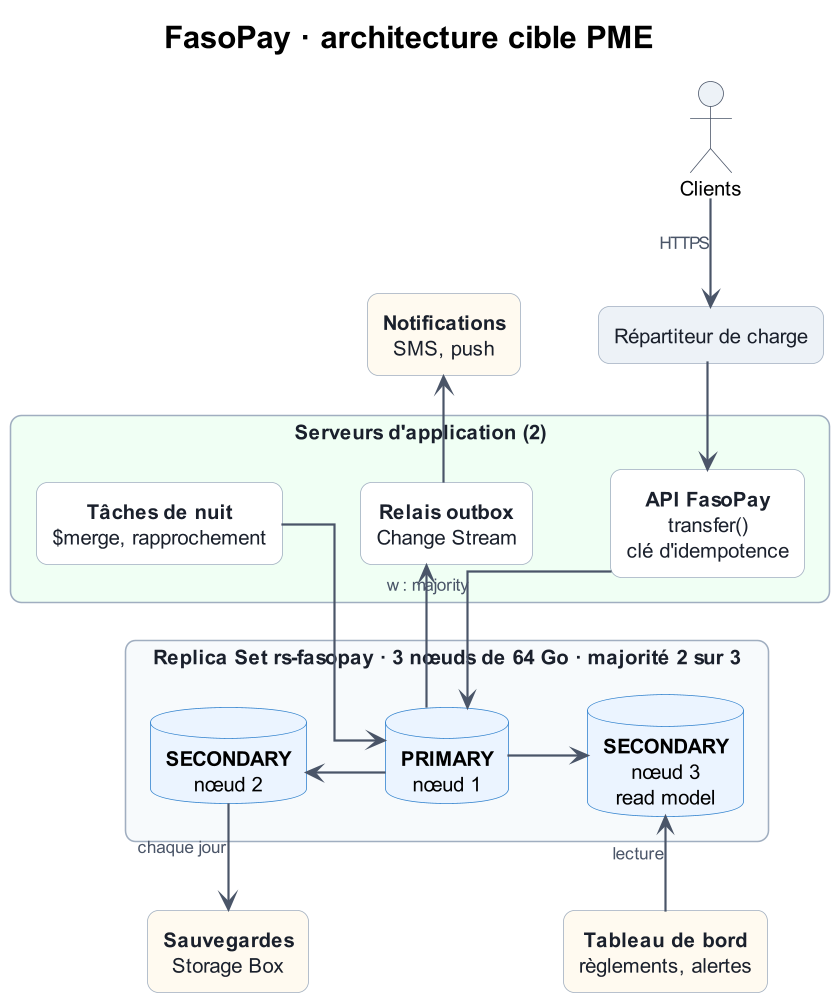
\includegraphics[width=0.56\linewidth]{diagramme-architecture.png}
		\caption{Architecture cible PME de FasoPay.}
	\end{figure}
	
	\textbf{Le chemin d'un virement :} l'API appelle \code{transfer()}, qui écrit les 6 documents en une transaction \code{w: "majority"} ; le relais envoie les notifications à partir de \code{outbox} (bonus B2) ; chaque nuit, un \code{$merge} recalcule le read model, lu sur un secondary, et le ledger est rapproché des soldes (E1).
	
	\subsection{Composants retenus, et le chiffre qui rend chacun nécessaire}
	\begin{center}\small
		\begin{tabularx}{\linewidth}{@{}P{4.1cm}L@{}}
			\toprule
			\textbf{Composant} & \textbf{Le chiffre qui le rend nécessaire} \\
			\midrule
			Replica Set de 3 nœuds & RPO 0 et 99,95 \% : 0 écriture perdue sur panne du primary, contre 97 en \code{w: 1} \\
			Nœuds de 64 Go de RAM & working set de 25,9 Go pour un cache de 31,5 Go (22 \% de marge) \\
			2 × 1 To NVMe en RAID 1 & 198,5 Go par an ; 2 ans gardés en ligne = 397 Go sur 700 Go utilisables (57 \%), archives au-delà \\
			\code{transfer()} avec clé d'idempotence & 21 clés rejouées et 65 rejeux (E4) ; sans clé, 633 025 FCFA débités en trop \\
			Client réglé à 1 s, \code{retryWrites} & interruption d'une panne ramenée de 21,2 s à 10,6 s \\
			Read model \code{ca_marchands} & 615 Mo de données nouvelles par jour : un \code{$merge} quotidien suffit, et le primary (330 virements/s mesurés pour 2 400 nécessaires) n'est pas sollicité \\
			Rapprochement nocturne & 6 soldes incohérents, 138 000 FCFA d'écart absolu (E1) \\
			Alertes plafond → \code{fraud_alerts} & 5 wallets qui découpent leurs transferts (E2) \\
			Relais outbox par Change Stream & un seul consommateur des événements ; 0 perdu, 0 doublon après \code{kill -9} (B2) \\
			Sauvegardes hors des nœuds & une suppression par erreur est répliquée en millisecondes : il faut une copie et l'oplog pour revenir avant l'erreur \\
			2 serveurs d'application & un seul rendrait inutile la disponibilité du Replica Set \\
			\bottomrule
		\end{tabularx}
	\end{center}
	
	\subsection{Composants écartés, avec le seuil qui les ferait revenir}
	\begin{center}\small
		\begin{tabularx}{\linewidth}{@{}P{2.6cm}LL@{}}
			\toprule
			\textbf{Composant} & \textbf{Pourquoi pas aujourd'hui} & \textbf{Nous le réintroduisons quand…} \\
			\midrule
			Sharding & 400 M tx/an, working set à 40 \% de la RAM & 490 M tx/an (working set à 50 \% de 64 Go), ou écritures au-delà de 50 \% du primary au test de charge \\
			Kafka & un seul consommateur, servi par un Change Stream & un 2\textsuperscript{e} consommateur indépendant doit relire les événements au-delà de l'oplog, ou le relais prend plus de 60 s de retard au pic \\
			Spark / Data Lake & 615 Mo par jour ; E3 en 23 ms & plus de 1 To à transformer par cycle, ou des sources hors MongoDB à croiser \\
			Redis (solde) & 3 M soldes = 0,43 Go en cache, lecture par index unique en 0 ms médiane (Q3) ; un cache créerait un second solde qui peut diverger & lecture de solde au-delà de 20 ms au p99 sous charge, ou plus de 20 000 lectures/s \\
			Lambda & pas de double besoin temps réel + recalcul lourd & les deux besoins à la fois \\
			Nœuds de 128 Go & 27 octets par entrée d'index & index au-delà de 45 octets par entrée, ou working set au-delà de 50 \% de la RAM \\
			\bottomrule
		\end{tabularx}
	\end{center}
	
	\subsection{Sécurité et conformité}
	\textbf{Authentification et rôles minimaux, prouvés.} Sur un serveur démarré avec authentification obligatoire, nous avons créé trois rôles, un par usage, et testé chaque utilisateur sur ce qu'il doit et ne doit pas pouvoir faire : \textbf{18 vérifications sur 18} (\preuve{07-securite.txt}).
	\begin{center}\small
		\begin{tabularx}{\linewidth}{@{}P{3.6cm}LL@{}}
			\toprule
			\textbf{Rôle} & \textbf{Peut} & \textbf{Ne peut pas (refusé, code 13)} \\
			\midrule
			\code{fasopay_application} & insérer transactions, lignes de ledger et événements ; mettre à jour un solde & \textbf{modifier ou supprimer une ligne de ledger}, supprimer un wallet, lire le read model \\
			\code{fasopay_relais} & lire et marquer les événements \code{outbox}, écrire une notification & modifier un solde, lire le ledger \\
			\code{fasopay_tableau} & lire le read model & lire les transactions, écrire \\
			\bottomrule
		\end{tabularx}
	\end{center}
	Le ledger devient ainsi un journal en \textbf{ajout seul} : même une API compromise ne peut pas réécrire l'historique de l'argent.
	
	\textbf{Chiffrement.} En transit : TLS\gl{68} partout (clients, API, et entre les nœuds avec \code{net.tls.mode: requireTLS}). Au repos : le moteur de stockage chiffré n'existe que dans l'édition Enterprise de MongoDB ; avec l'édition Community, nous chiffrons les disques au niveau du système et les sauvegardes avant leur envoi. \textbf{Journal d'audit :} la documentation de MongoDB 8.0 ne le décrit que pour Enterprise et Atlas ; nous nous appuyons sur le ledger en ajout seul, le journal du serveur conservé hors des nœuds et un utilisateur par rôle. \textbf{Conservation :} les lignes de ledger ne sont jamais supprimées ; au-delà de 2 ans, elles passent dans une archive chiffrée. Nous ne fixons pas nous-mêmes la durée légale.
	
	\textbf{Autorités à consulter :} la \textbf{Commission de l'Informatique et des Libertés (CIL\gl{12})} du Burkina Faso, autorité de protection des données personnelles, notamment parce que nos serveurs seraient hors du pays ; et la \textbf{BCEAO\gl{7}}, qui délivre l'agrément des émetteurs de monnaie électronique dans l'UEMOA\gl{71}.
	
	\needspace{12\baselineskip}
	\subsection{Coût indicatif mensuel}
	Prix publics hors taxes relevés en novembre 2026 chez Hetzner, au taux fixe de 1 € = 655,957 FCFA.
	\begin{center}\small
		\begin{tabularx}{\linewidth}{@{}Lrr@{}}
			\toprule
			\textbf{Poste} & \textbf{€ HT / mois} & \textbf{soit FCFA} \\
			\midrule
			3 serveurs dédiés EX63 (64 Go ECC, 2 × 1 To NVMe) : le Replica Set & 447,00 & 293 213 \\
			Storage Box 5 To : sauvegardes et archives & 10,90 & 7 150 \\
			2 serveurs cloud CX33 avec IPv4 : API, relais, tâches, surveillance & 17,98 & 11 794 \\
			Répartiteur de charge LB11 avec IPv4 & 7,49 & 4 913 \\
			\midrule
			\textbf{Total} & \textbf{483,37} & \textbf{317 070} \\
			\bottomrule
		\end{tabularx}
	\end{center}
	Plus 222 € d'installation une seule fois, soit environ 145 622 FCFA. \textbf{Hypothèses :} prix sans remise et susceptibles de changer ; serveur EX44 écarté (59 €) car sans mémoire ECC ; nœuds dans des centres de données différents ; hors personnel, SMS, licence Enterprise, et hors hébergement au Burkina Faso si la CIL ou la BCEAO l'exigent (nous n'avons pas de prix vérifié à donner) ; latence Ouagadougou--Europe non mesurée.
	
	\textbf{ADR-003 (décision).} Cible PME : un Replica Set de 3 nœuds de 64 Go, un read model et un relais outbox par Change Stream\gl{10}, \textbf{sans Kafka, Spark, Redis ni sharding à 18 mois}. Rejetés : l'architecture Enterprise (au moins 15 machines au lieu de 3, sans qu'aucun seuil ne soit franchi), un serveur seul (incompatible avec 99,95 \%), Redis devant les soldes et Kafka dès le démarrage. À revoir aux seuils du tableau des écartés, et d'abord au test de charge. ADR complet dans \code{adr/ADR-003.md}.
	
	\retenir{trois serveurs de 64 Go, un read model et un relais suffisent à la cible, pour environ 483 € HT par mois. Kafka, Spark, Redis et le sharding sont écartés aujourd'hui, chacun avec le chiffre qui le ferait revenir.}
	
	% =====================================================
	% 10. SYNTHÈSE CTO
	% =====================================================
	\clearpage
	\section{Synthèse CTO : 5 priorités pour les 12 prochains mois}\sectionmark{Synthèse CTO}
	
	Cette page résume le rapport pour le CTO : ce qu'il faut faire dans les 12 prochains mois, dans l'ordre, et ce qu'il ne faut pas faire.
	
	\textbf{Notre verdict.} FasoPay n'a pas besoin d'une plateforme de données, mais d'un Replica Set de 3 nœuds bien réglé, d'un \code{transfer()} utilisé partout et d'un contrôle quotidien de l'argent, pour environ \textbf{483 € HT par mois, soit environ 317 070 FCFA}.
	
	\begin{enumerate}[leftmargin=*]
		\item \textbf{Réparer la confiance dans les soldes (mois 1).} Corriger les 6 soldes incohérents (138 000 FCFA d'écart absolu) par des écritures d'ajustement, en partant du ledger qui fait foi, puis lancer chaque nuit le rapprochement. \emph{Réussite :} 0 écart chaque matin, et tout nouvel écart vu par la finance avant le support.
		\item \textbf{Faire passer 100 \% des flux d'argent par \code{transfer()} (mois 1 à 3)}, avec une clé d'idempotence fixée par le client. C'est la réponse aux rejeux de l'incident du 10 avril : un seul débit pour 3 rejeux, 30 virements sur 50 en concurrence, jamais de solde négatif. \emph{Réussite :} 0 doublon, 0 solde négatif.
		\item \textbf{Mettre en production le Replica Set sûr (mois 2 à 4) :} 3 nœuds de 64 Go sur des sites différents, \code{w: "majority"} pour l'argent, client réglé à 1 s, sauvegardes avec restauration \textbf{testée}, TLS, disques chiffrés et les trois rôles minimaux.
		\item \textbf{Outiller la conformité et la finance (mois 3 à 6) :} alerte automatique sur le découpage sous le plafond (5 wallets aujourd'hui), read model pour le tableau de bord et les règlements, relais outbox pour les notifications ; consulter dès maintenant la CIL et intégrer les exigences de la BCEAO.
		\item \textbf{Mesurer avant de grandir (mois 4 à 12) :} test de charge sur le matériel cible (il faut 2 400 virements/s, nous en mesurons 330 sur notre ordinateur portable), puis suivi mensuel des seuils : working set au-delà de 50 \% de la RAM, index au-delà de 45 octets par entrée, volume vers 490 M tx/an. La shard key est déjà choisie.
	\end{enumerate}
	
	\textbf{Ce que nous ne ferons PAS}
	\begin{center}\small
		\begin{tabularx}{\linewidth}{@{}P{3.6cm}LL@{}}
			\toprule
			\textbf{Nous ne ferons pas} & \textbf{Parce que (nos chiffres)} & \textbf{Sauf si} \\
			\midrule
			Kafka & un seul consommateur des événements & un 2\textsuperscript{e} consommateur doit les relire \\
			Spark ou un Data Lake & 615 Mo nouveaux par jour, E3 en 23 ms & plus de 1 To par cycle \\
			Redis devant les soldes & 0,43 Go en cache, lecture par index unique en 0 ms (Q3) & p99 au-delà de 20 ms sous charge \\
			Sharding & 400 M tx/an, working set à 40 \% de la RAM & 490 M tx/an ou test de charge insuffisant \\
			Modifier ou supprimer le ledger & le ledger est la preuve de l'argent & jamais \\
			Changer de base de données & MongoDB couvre transactions, réplication, Change Streams et agrégats, et tout notre POC tourne dessus & jamais sans mesure qui le justifie \\
			\bottomrule
		\end{tabularx}
	\end{center}
	
	\textbf{La décision à prendre maintenant :} valider la cible PME (ADR-003) et commander le test de charge sur le matériel cible ; c'est le seul chiffre qui pourrait changer cette architecture.
	
	% =====================================================
	% 11. BONUS B2
	% =====================================================
	\section{Bonus B2 · Relais Outbox par Change Stream}\sectionmark{Bonus B2 · Relais Outbox}
	
	Après un virement, le client doit recevoir sa notification (SMS ou application) une fois et une seule, même si le programme qui l'envoie tombe en panne. C'est le rôle du relais que nous avons construit et tué volontairement en pleine activité.
	
	\code{transfer()} écrit l'événement \code{outbox} dans la même transaction que le virement : un virement validé a toujours son événement. Il reste à l'\textbf{envoyer} sans en perdre un et sans en envoyer deux, même si le relais meurt n'importe quand. Notre relais (\code{code/B2-relais.js}) ouvre un Change Stream sur \code{outbox} avec un filtre appliqué \textbf{par le serveur} (seules les insertions \code{PENDING} lui parviennent). Pour chaque événement, dans cet ordre : (1) il écrit la notification avec \textbf{le même \code{_id} que l'événement} ; (2) il passe l'événement à \code{SENT} ; (3) il sauvegarde le \textbf{resume token\gl{56}}. Au redémarrage, il reprend avec \code{resumeAfter}\gl{57}.
	
	\begin{center}\small
		\begin{tabularx}{\linewidth}{@{}P{4.6cm}LL@{}}
			\toprule
			\textbf{Scénario} & \textbf{Ce qui s'est passé} & \textbf{Résultat} \\
			\midrule
			\code{kill -9} au milieu de 1 000 virements & relais tué après 324 notifications ; 410 événements s'accumulent pendant 3 s ; reprise « après 323 » & 1 relivraison reconnue ; 1 000 événements, 1 000 notifications, \textbf{0 perdu, 0 doublon} \\
			Arrêt juste après la 5\textsuperscript{e} notification, avant \code{SENT} et avant le resume token & 1 005 notifications pour 1 004 événements \code{SENT} au moment de l'arrêt & 1 relivraison reconnue ; 1 020 / 1 020, \textbf{0 perdu, 0 doublon} \\
			\bottomrule
		\end{tabularx}
	\end{center}
	Chaque scénario se termine par 6 vérifications, toutes OK (\preuve{B2-relais-outbox.txt}). Le \code{kill -9}\gl{33} est tombé, par hasard, dans la fenêtre dangereuse ; le second scénario la provoque exprès, pour que la preuve ne dépende pas du hasard.
	
	\textbf{Pourquoi « au moins une fois ».} Le resume token est sauvegardé \emph{après} la notification : si le relais meurt entre les deux, le Change Stream relivre l'événement au redémarrage. Rien n'est perdu, mais un événement peut arriver deux fois. Sauvegarder le resume token avant ferait l'inverse, et perdrait un événement à chaque arrêt dans cette fenêtre : pour de l'argent, nous préférons recevoir deux fois que jamais.
	
	\textbf{Ce qui rend le résultat « exactement une fois ».} La notification porte le même \code{_id} que l'événement, et \code{_id} est unique : à la relivraison, \code{upsert}\gl{73} avec \code{$setOnInsert} trouve la notification déjà écrite et ne change rien. La livraison est « au moins une fois », l'effet « exactement une fois » : c'est le principe de la clé d'idempotence de \code{transfer()}, appliqué au relais. \textbf{Limites :} au-delà de la fenêtre de l'oplog, la reprise doit repartir des événements encore \code{PENDING} ; un vrai fournisseur de SMS devrait recevoir lui aussi l'\code{_id} comme clé.
	
	% =====================================================
	% 12. CONCLUSION
	% =====================================================
	\section{Conclusion et limites du POC}
	
	Les quatre demandes du CTO ont une réponse prouvée. \textbf{Le modèle} rejette ce qui est faux et tient la comptabilité en partie double. \textbf{L'enquête} trouve les 6 soldes divergents et chiffre leur écart, identifie 5 wallets qui découpent leurs transferts, et montre que l'idempotence a tenu pendant l'incident du 10 avril. \textbf{Les virements} ne peuvent plus ni doubler ni se perdre : nous l'avons prouvé par l'abort, la concurrence, trois pannes réelles et un relais tué en pleine rafale. \textbf{L'architecture} est proportionnée à nos chiffres, chaque composant écarté a son seuil de retour, et elle coûte environ 317 070 FCFA par mois.
	
	\textbf{Ce que notre POC\gl{47} ne prouve pas}, et que nous ne prétendons pas : le débit au pic (330 virements/s sur notre ordinateur portable pour 2 400 nécessaires, à trancher par un test de charge) ; la taille des index à 400 millions de documents (d'où notre seuil de 45 octets) ; les performances d'un vrai réseau, puisque nos nœuds et nos shards partagent une machine ; la cause des 6 soldes divergents, dont le « lost update » n'est qu'une explication possible ; et les exigences de la CIL et de la BCEAO.
	
	% =====================================================
	% ANNEXES
	% =====================================================
	\clearpage
	\appendix
	% ---------- Page de titre des annexes ----------
	\thispagestyle{empty}
	\addcontentsline{toc}{part}{Annexes}
	\vspace*{\fill}
	\begin{center}
		{\color{bleufaso}\rule{0.6\linewidth}{1.2pt}\par}
		\vspace{0.6cm}
		{\Huge\bfseries Annexes\par}
		\vspace{0.6cm}
		{\color{bleufaso}\rule{0.6\linewidth}{1.2pt}\par}
		\vspace{1.2cm}
		{\large
			\begin{tabular}{@{}ll@{}}
				Annexe A & Feuille de dimensionnement \\[3pt]
				Annexe B & Journal de montage \\[3pt]
				Annexe C & Code \\[3pt]
				Annexe D & Preuves \\[3pt]
				Annexe E & Déclaration d'usage de l'IA \\[3pt]
				Annexe F & Contribution de chaque membre \\[3pt]
				Annexe G & Lexique \\
			\end{tabular}\par}
	\end{center}
	\vspace*{\fill}
	\clearpage
	
	\section*{Annexe A · Feuille de dimensionnement}
	\addcontentsline{toc}{section}{Annexe A · Feuille de dimensionnement}
	\markboth{Annexe A · Feuille de dimensionnement}{}
	\begingroup\small\sloppy
	Groupe : 07 · empreinte (\texttt{datasetSha256}, début) : 9b0b9a40
	
	Unités : 1 Mo = 1 000 000 octets, 1 Go = 1 000 000 000 octets. Mesures : \texttt{preuves/00-dimensionnement.txt} (commandes dans \texttt{code/00-dimensionnement.js}).
	
	\subsection*{Cible à 18 mois (donnée du sujet)}
	
	3 000 000 wallets · 400 000 000 transactions/an · pic 1 200 tx/s · disponibilité 99,95 \% · RPO 0
	
	\subsection*{1. Mesures sur notre jeu (POC)}
	
	\begin{longtable}[]{@{}
			>{\raggedright\arraybackslash}p{(\columnwidth - 8\tabcolsep) * \real{0.2000}}
			>{\raggedright\arraybackslash}p{(\columnwidth - 8\tabcolsep) * \real{0.2000}}
			>{\raggedright\arraybackslash}p{(\columnwidth - 8\tabcolsep) * \real{0.2000}}
			>{\raggedright\arraybackslash}p{(\columnwidth - 8\tabcolsep) * \real{0.2000}}
			>{\raggedright\arraybackslash}p{(\columnwidth - 8\tabcolsep) * \real{0.2000}}@{}}
		\toprule\noalign{}
		\begin{minipage}[b]{\linewidth}\raggedright
			Collection
		\end{minipage} & \begin{minipage}[b]{\linewidth}\raggedright
			Documents
		\end{minipage} & \begin{minipage}[b]{\linewidth}\raggedright
			Taille BSON moyenne (octets)
		\end{minipage} & \begin{minipage}[b]{\linewidth}\raggedright
			Données (Mo)
		\end{minipage} & \begin{minipage}[b]{\linewidth}\raggedright
			Index (Mo)
		\end{minipage} \\
		\midrule\noalign{}
		\endhead
		\bottomrule\noalign{}
		\endlastfoot
		transactions & 60 000 & 253,02 & 15,18 & 5,05 \\
		ledger\_entries & 141 939 & 130,19 & 18,48 & 7,48 \\
		wallets & 2 000 & 144 & 0,29 & 0,11 \\
	\end{longtable}
	
	Les tailles moyennes viennent de \texttt{\$bsonSize} sur toute la collection ; un échantillon aléatoire de 1 000 documents donne 252,44 (transactions) et 130,30 (ledger). « Données » est la taille BSON non compressée (\texttt{size}) ; sur disque, la compression ramène les transactions à 7,98 Mo et le ledger à 9,27 Mo (\texttt{storageSize}). Les index sont ceux de la Partie 3 (3 sur \texttt{transactions}, 2 sur \texttt{ledger\_entries}).
	
	Lignes de ledger par transaction (mesuré) : 2,36565 (141 939 / 60 000), dont 1,19808 jambes de wallet (71 885 / 60 000).
	
	Documents écrits par transaction métier (mesuré sur les 56 484 transactions qui ont un ledger) : 1 transaction + 2,513 lignes de ledger + 1,273 soldes de wallet + 1 outbox = 5,79 en moyenne. Par type : P2P 6,03, CASH\_IN 5, CASH\_OUT 6, BILL 6,02, MERCHANT\_PAY 6,03.
	
	\subsection*{2. Extrapolation}
	
	\begin{longtable}[]{@{}
			>{\raggedright\arraybackslash}p{(\columnwidth - 4\tabcolsep) * \real{0.3333}}
			>{\raggedright\arraybackslash}p{(\columnwidth - 4\tabcolsep) * \real{0.3333}}
			>{\raggedright\arraybackslash}p{(\columnwidth - 4\tabcolsep) * \real{0.3333}}@{}}
		\toprule\noalign{}
		\begin{minipage}[b]{\linewidth}\raggedright
			Grandeur
		\end{minipage} & \begin{minipage}[b]{\linewidth}\raggedright
			Calcul (formule + nombres)
		\end{minipage} & \begin{minipage}[b]{\linewidth}\raggedright
			Résultat
		\end{minipage} \\
		\midrule\noalign{}
		\endhead
		\bottomrule\noalign{}
		\endlastfoot
		Volume brut/an (données) & 400 M × (253,02 + 2,36565 × 130,19) = 400 M × 561,02 octets & 224,4 Go \\
		Facteur d'index retenu (et pourquoi) & (33 661 042 + 12 529 664) / 33 661 042 : données puis index de \texttt{transactions} et \texttt{ledger\_entries}, mesurés après les index de la Partie 3. Ces deux collections portent 98 \% des données. & ×1,37 \\
		Volume/an avec index & 224,4 Go × 1,3723 & 307,9 Go \\
		Écritures/s au pic & 1 200 × 6 documents (1 transaction + 2 lignes de ledger + 2 soldes + 1 outbox, ADR-001) ; en plus 8 entrées d'index par virement (3 sur \texttt{transactions}, 4 sur \texttt{ledger\_entries}, 1 sur \texttt{outbox}) & 7 200 documents/s et 9 600 entrées d'index/s \\
		Working set (30 jours chauds + index chauds) & 400 M × 30 / 365 = 32,88 M transactions × 561,02 o = 18,44 Go ; index chauds 18,44 × 0,3723 = 6,87 Go ; 3 M wallets × 144 o = 0,43 Go ; index des wallets 3 M × 55,3 o = 0,17 Go & 25,9 Go \\
		RAM par nœud (cache WiredTiger ≈ 50 \% de (RAM − 1 Go)) & 50 \% × (RAM − 1) ≥ 25,9 donc RAM ≥ 2 × 25,9 + 1 = 52,8 Go : nœud de 64 Go (cache 31,5 Go, marge 22 \%) & 64 Go \\
		Disque par nœud et horizon avant saturation & données sur disque : 224,4 Go × 0,5124 (compression mesurée : 17 248 256 / 33 661 042) = 115,0 Go ; index : 224,4 × 0,3723 = 83,5 Go ; total 198,5 Go/an ; disque utilisable : 2 × 1 To en RAID 1 = 1 To, dont 70 \% = 700 Go ; 700 / 198,5 & 3,5 ans \\
		Facteur de pic & moyenne : 400 M ÷ (365 × 86 400 s) = 12,7 tx/s ; pic ÷ moyenne = 1 200 ÷ 12,7 & ×95 : nous dimensionnons sur le pic, pas sur la moyenne \\
		Rétention sur 5 ans & sur disque : 5 × 198,5 Go = 0,99 To ; non compressé, avec index : 5 × 307,9 Go = 1,54 To & ne tient pas sur 700 Go utilisables, et entre dans la zone de 1 à 2 To par Replica Set à partir de laquelle on envisage de répartir : nous archivons au-delà de 2 ans (2 × 198,5 = 397 Go, soit 57 \% du disque) \\
	\end{longtable}
	
	\subsection*{2 bis. Un chiffre qui contredit l'architecture : la taille des index}
	
	Mesuré : 12 529 664 octets d'index pour 463 878 entrées (3 index × 60 000 transactions + 2 index × 141 939 lignes), soit \textbf{27 octets par entrée}. C'est peu : à 60 000 documents, un index reste plus compact qu'à 400 millions. Une règle de prudence courante compte 40 à 60 octets par entrée (chapitre 11). Nous refaisons donc le calcul avec ces valeurs :
	
	\begin{longtable}[]{@{}
			>{\raggedright\arraybackslash}p{(\columnwidth - 8\tabcolsep) * \real{0.2000}}
			>{\raggedright\arraybackslash}p{(\columnwidth - 8\tabcolsep) * \real{0.2000}}
			>{\raggedright\arraybackslash}p{(\columnwidth - 8\tabcolsep) * \real{0.2000}}
			>{\raggedright\arraybackslash}p{(\columnwidth - 8\tabcolsep) * \real{0.2000}}
			>{\raggedright\arraybackslash}p{(\columnwidth - 8\tabcolsep) * \real{0.2000}}@{}}
		\toprule\noalign{}
		\begin{minipage}[b]{\linewidth}\raggedright
			Hypothèse
		\end{minipage} & \begin{minipage}[b]{\linewidth}\raggedright
			Index par transaction métier (7,73 entrées)
		\end{minipage} & \begin{minipage}[b]{\linewidth}\raggedright
			Index chauds (30 jours)
		\end{minipage} & \begin{minipage}[b]{\linewidth}\raggedright
			Working set
		\end{minipage} & \begin{minipage}[b]{\linewidth}\raggedright
			RAM nécessaire
		\end{minipage} \\
		\midrule\noalign{}
		\endhead
		\bottomrule\noalign{}
		\endlastfoot
		Mesuré (27 o) & 209 o & 6,9 Go & 25,9 Go & 52,8 Go : 64 Go suffit \\
		Prudence basse (40 o) & 309 o & 10,2 Go & 29,2 Go & 59,4 Go : 64 Go juste \\
		Prudence haute (60 o) & 464 o & 15,3 Go & 34,3 Go & 69,6 Go : \textbf{64 Go ne suffit plus} \\
	\end{longtable}
	
	Le nœud de 64 Go tient tant que les index restent sous \textbf{49 octets par entrée} : au-delà, le working set dépasse le cache de 31,5 Go. Nous gardons donc 64 Go comme base, avec un seuil de surveillance : si les index dépassent 45 octets par entrée en production, ou si le working set dépasse 50 \% de la RAM, nous passons à des nœuds de 128 Go. C'est une montée en gamme, pas un sharding.
	
	\subsection*{2 ter. Un deuxième chiffre qui contredit : le débit mesuré}
	
	Nous avons mesuré \texttt{transfer()} sur notre machine (Partie 4, \texttt{preuves/04-debit.txt}) : \textbf{125 virements/s} avec un client, \textbf{330 virements/s} avec 4 clients en parallèle (1 978 écritures de documents/s), p95 à 17 ms. La cible est de 1 200 virements/s au pic, et la règle que nous retenons demande que les écritures restent sous \textbf{50 \% de la capacité du primary} : il faudrait donc un primary capable d'environ \textbf{2 400 virements/s}, soit plus de 7 fois ce que nous mesurons.
	
	Ce chiffre ne condamne pas l'architecture, mais il ne la prouve pas non plus : la mesure a été faite sur un ordinateur portable, avec les clients sur la même machine que le serveur et un seul nœud. \textbf{Décision :} avant la mise en production, un test de charge sur le matériel cible est obligatoire. Si le primary n'y atteint pas 2 400 virements/s, nous montons d'abord en gamme (CPU, disques plus rapides) ; si cela ne suffit pas, nous répartissons les écritures (sharding, Partie 6).
	
	\subsection*{3. Verdict (une phrase chacun, avec un SEUIL chiffré)}
	
	Nous décidons chaque composant sur trois critères : le volume par Replica Set, la part de la RAM prise par le working set, et la part du débit du primary prise par les écritures. Pour Kafka, ce n'est pas le débit qui compte, mais le nombre de consommateurs indépendants et le besoin de rejeu.
	
	\begin{longtable}[]{@{}
			>{\raggedright\arraybackslash}p{(\columnwidth - 4\tabcolsep) * \real{0.3333}}
			>{\raggedright\arraybackslash}p{(\columnwidth - 4\tabcolsep) * \real{0.3333}}
			>{\raggedright\arraybackslash}p{(\columnwidth - 4\tabcolsep) * \real{0.3333}}@{}}
		\toprule\noalign{}
		\begin{minipage}[b]{\linewidth}\raggedright
			Question
		\end{minipage} & \begin{minipage}[b]{\linewidth}\raggedright
			Réponse
		\end{minipage} & \begin{minipage}[b]{\linewidth}\raggedright
			Seuil de bascule (chiffré, avec votre ordre de grandeur)
		\end{minipage} \\
		\midrule\noalign{}
		\endhead
		\bottomrule\noalign{}
		\endlastfoot
		Un seul replica set suffit-il ? & Oui à 18 mois : 0,31 To par an non compressé (sous la zone de 1 à 2 To) ; working set de 25,9 Go sur 64 Go, soit 40 \% de la RAM (54 \% dans l'hypothèse prudente de la section 2 bis) ; pour les 7 200 écritures par seconde au pic, nous avons mesuré 330 virements/s sur notre ordinateur portable (section 2 ter) : le critère n'est pas encore vérifié sur le matériel cible. & Working set au-delà de 50 \% de la RAM ; ou plus de 1 à 2 To par replica set ; ou écritures au-delà de 50 \% du débit du primary, mesuré par un test de charge sur le matériel cible (il faut au moins 2 400 virements/s). \\
		Sharding ? & Non : aucun des trois critères n'est franchi à 18 mois. Nous ne le déclencherons que sur cette feuille et un test de charge. & Sur des nœuds de 64 Go : 490 M tx/an, quand le working set atteint 50 \% de la RAM, soit la taille du cache. En volume : 1 To non compressé atteint en 3,2 ans, 2 To en 6,5 ans. \\
		Kafka ? & Non au démarrage : un seul consommateur des événements \texttt{outbox} (le relais de notifications), qu'un Change Stream avec resume token suffit à servir. & Dès qu'un \textbf{deuxième consommateur indépendant} doit relire les événements au-delà de la fenêtre de l'oplog (par exemple la détection de fraude ou la comptabilité), ou qu'il faut un tampon devant le pic. Probable à la cible : nous le tranchons en Partie 7. \\
		Spark / Data Lake ? & Non : 224,4 Go de données par an, soit environ 615 Mo par jour ; un \texttt{\$merge} quotidien vers un read model suffit. E3 prend 23 ms sur le POC (\texttt{03-explain.txt}). & Plusieurs To à transformer par cycle, ou des sources hétérogènes hors MongoDB (opérateurs télécom, banques partenaires). \\
		Redis pour le solde ? & Non : les 3 M soldes pèsent 0,43 Go et tiennent dans le cache ; une lecture par index unique, comme celle d'un solde par \texttt{\_id}, prend 0 ms en médiane (Q3, \texttt{03-explain.txt}). Nous n'ajoutons pas de cache sans mesure qui le justifie. & Une lecture de solde au-delà de 20 ms au p99, mesurée sous charge, ou plus de 20 000 lectures de solde par seconde soutenues. \\
		Lambda ? & Non : nous n'avons pas de besoin cumulé de temps réel \textbf{et} de recalcul historique lourd. & Les deux besoins à la fois, sans qu'un seul moteur puisse les servir. \\
	\end{longtable}
	
	\subsection*{4. Hypothèses (liste)}
	
	\textbf{Mesurées sur le POC, puis extrapolées :}
	1. Tailles moyennes : 253,02 octets par transaction, 130,19 par ligne de ledger, 144 par wallet ; 2,36565 lignes de ledger par transaction. Nous supposons qu'elles restent les mêmes à 3 M wallets (identifiants de même forme).
	2. Compression sur disque (0,5124) et facteur d'index (0,3723), mesurés sur le POC et supposés constants. Le facteur d'index est probablement optimiste : voir la section 2 bis.
	3. Écritures par transaction métier : 6 dans le cas le plus lourd, 5,79 en moyenne mesurée.
	
	\textbf{Non testées :}
	4. Unités décimales : 1 Mo = 10⁶ octets, 1 Go = 10⁹ octets.
	5. Fenêtre chaude de 30 jours, trafic réparti sur l'année (30 / 365 du volume annuel). Un pic de 2 h chaque 1er du mois représenterait 8,64 M transactions par mois, soit 26 \% du volume : nous supposons qu'il reste dans le mois chaud.
	6. Nœud de référence : 64 Go de RAM, deux disques de 1 To en RAID 1 (1 To), dont 70 \% utilisables, soit 700 Go ; l'oplog n'est pas compté.
	7. Les 3 M wallets sont tous dans le working set ; \texttt{customers} (0,46 Go) et \texttt{merchants} (0,013 Go) n'y sont pas.
	8. Les documents \texttt{outbox} sont supprimés après envoi : ils n'entrent pas dans le volume annuel (un document pèse 109 octets, mesuré).
	9. Volume constant de 400 M tx/an ; archivage des données de plus de 2 ans.
	10. Taille des index par entrée : 27 octets mesurés, 40 à 60 en hypothèse prudente (section 2 bis).
	11. Débit d'écriture d'un nœud : mesuré sur un ordinateur portable seulement (125 virements/s avec 1 client, 330 avec 4) ; la capacité d'un serveur de production n'est pas testée (section 2 ter).
	
	\endgroup
	
	\clearpage
	\section*{Annexe B · Journal de montage}
	\addcontentsline{toc}{section}{Annexe B · Journal de montage}
	\markboth{Annexe B · Journal de montage}{}
	Les commandes qui construisent nos environnements, dans l'ordre, telles que nous les avons tapées. Le journal complet, avec l'objectif de chaque étape, le résultat attendu et la date de chaque preuve, est dans \texttt{docs/journal-montage.md} (dans le ZIP).
	\begingroup\small\sloppy
	\lstset{basicstyle=\ttfamily\scriptsize}
	\subsection*{1. Environnement de départ}
	\begin{lstlisting}
		git --version
	\end{lstlisting}
	\begin{lstlisting}
		docker --version
	\end{lstlisting}
	\begin{lstlisting}
		docker info --format "{{.MemTotal}}"
	\end{lstlisting}
	\subsection*{2. Données du groupe et vérification}
	\begin{lstlisting}
		Get-ChildItem data\*.ndjson | ForEach-Object {
			"{0}  {1}  {2}" -f (Get-FileHash $_.FullName -Algorithm SHA256).Hash.ToLower().Substring(0,8), $_.Name, $_.Length
		}
	\end{lstlisting}
	\subsection*{3. Serveur MongoDB (D1)}
	\begin{lstlisting}
		docker run -d --name mongo-rs1 -p 27017:27017 -v mongo-rs1-data:/data/db mongo:8.0 --replSet rs0
	\end{lstlisting}
	\begin{lstlisting}
		docker exec mongo-rs1 mongod --version
	\end{lstlisting}
	\begin{lstlisting}
		docker exec mongo-rs1 mongosh --version
	\end{lstlisting}
	\subsection*{4. Initialisation du Replica Set (D1)}
	\begin{lstlisting}
		docker exec mongo-rs1 mongosh --eval "rs.initiate({_id: 'rs0', members: [{_id: 0, host: 'localhost:27017'}]})"
	\end{lstlisting}
	\subsection*{5. Vérification du Replica Set (D1)}
	\begin{lstlisting}
		docker exec mongo-rs1 mongosh --eval "rs.status()"
	\end{lstlisting}
	\begin{lstlisting}
		docker exec mongo-rs1 date -u
	\end{lstlisting}
	\begin{lstlisting}
		docker exec mongo-rs1 mongosh --eval "rs.status()"
	\end{lstlisting}
	\subsection*{6. Copie des données dans le conteneur (D2)}
	\begin{lstlisting}
		docker cp data mongo-rs1:/tmp/data
	\end{lstlisting}
	\subsection*{7. Import des collections (D2)}
	\begin{lstlisting}
		docker exec mongo-rs1 mongoimport --db fasopay_tp --collection customers --file /tmp/data/customers.ndjson
	\end{lstlisting}
	\begin{lstlisting}
		docker exec mongo-rs1 mongoimport --db fasopay_tp --collection wallets --file /tmp/data/wallets.ndjson
	\end{lstlisting}
	\begin{lstlisting}
		docker exec mongo-rs1 mongoimport --db fasopay_tp --collection merchants --file /tmp/data/merchants.ndjson
	\end{lstlisting}
	\begin{lstlisting}
		docker exec mongo-rs1 mongoimport --db fasopay_tp --collection transactions --file /tmp/data/transactions.ndjson
	\end{lstlisting}
	\begin{lstlisting}
		docker exec mongo-rs1 mongoimport --db fasopay_tp --collection ledger_entries --file /tmp/data/ledger_entries.ndjson
	\end{lstlisting}
	\subsection*{8. Comptage des collections (preuve D2)}
	\begin{lstlisting}
		docker exec mongo-rs1 mongosh fasopay_tp --quiet --eval "db.getCollectionNames().forEach(function(c){ print(c + ' : ' + db[c].countDocuments()) })"
	\end{lstlisting}
	\begin{lstlisting}
		docker exec mongo-rs1 date -u
	\end{lstlisting}
	\begin{lstlisting}
		docker exec mongo-rs1 mongosh fasopay_tp --quiet --eval "db.getCollectionNames().forEach(function(c){ print(c + ' : ' + db[c].countDocuments()) })"
	\end{lstlisting}
	\subsection*{9. Vérification des données (D3)}
	\begin{lstlisting}
		docker exec mongo-rs1 mongosh fasopay_tp --quiet --eval "db.transactions.aggregate([{`$group:{_id:null, total:{`$sum:'`$amount'}}}]).toArray()"
	\end{lstlisting}
	\begin{lstlisting}
		docker exec mongo-rs1 mongosh fasopay_tp --quiet --eval "db.transactions.aggregate([{`$match:{status:'COMPLETED'}},{`$group:{_id:null, total:{`$sum:'`$amount'}}}]).toArray()"
	\end{lstlisting}
	\begin{lstlisting}
		docker exec mongo-rs1 mongosh fasopay_tp --quiet --eval "db.wallets.aggregate([{`$group:{_id:null, total:{`$sum:'`$balance'}}}]).toArray()"
	\end{lstlisting}
	\begin{lstlisting}
		Get-ChildItem data\*.ndjson | ForEach-Object { "{0}  {1}" -f (Get-FileHash $_.FullName -Algorithm SHA256).Hash.ToLower(), $_.Name }
	\end{lstlisting}
	\begin{lstlisting}
		docker exec mongo-rs1 date -u
	\end{lstlisting}
	\subsection*{10. Création des collections vides (D4)}
	\begin{lstlisting}
		docker exec mongo-rs1 mongosh fasopay_tp --quiet --eval "db.createCollection('outbox')"
		docker exec mongo-rs1 mongosh fasopay_tp --quiet --eval "db.createCollection('fraud_alerts')"
		
		docker exec mongo-rs1 mongosh fasopay_tp --quiet --eval "db.getCollectionNames().sort()"
	\end{lstlisting}
	\subsection*{11. Vérification des types après l'import}
	\begin{lstlisting}
		docker exec -it mongo-rs1 mongosh fasopay_tp
	\end{lstlisting}
	\begin{lstlisting}
		db.transactions.aggregate([{$group: {_id: {amount: {$type: "$amount"}, createdAt: {$type: "$createdAt"}}, n: {$sum: 1}}}])
		db.transactions.aggregate([{$group: {_id: {fee: {$type: "$fee"}, completedAt: {$type: "$completedAt"}}, n: {$sum: 1}}}])
		db.wallets.aggregate([{$group: {_id: {balance: {$type: "$balance"}, dailyLimit: {$type: "$dailyLimit"}, version: {$type: "$version"}, updatedAt: {$type: "$updatedAt"}}, n: {$sum: 1}}}])
		db.ledger_entries.aggregate([{$group: {_id: {amount: {$type: "$amount"}, balanceAfter: {$type: "$balanceAfter"}, walletId: {$type: "$walletId"}, createdAt: {$type: "$createdAt"}}, n: {$sum: 1}}}])
		db.customers.aggregate([{$group: {_id: {kycLevel: {$type: "$kycLevel"}, createdAt: {$type: "$createdAt"}}, n: {$sum: 1}}}])
		db.merchants.aggregate([{$group: {_id: {mcc: {$type: "$mcc"}, feePct: {$type: "$feePct"}, location: {$type: "$location"}, createdAt: {$type: "$createdAt"}}, n: {$sum: 1}}}])
	\end{lstlisting}
	\subsection*{12. Validateurs de la Partie 1}
	Commandes tapées dans la session : \code{code/01-validateurs.js}.
	\begin{lstlisting}
		docker exec -it mongo-rs1 mongosh fasopay_tp
	\end{lstlisting}
	\subsection*{13. Mesures pour la modélisation (Partie 1)}
	Commandes tapées dans la session : \code{code/01-mesures-modelisation.js}.
	\begin{lstlisting}
		docker exec -it mongo-rs1 mongosh fasopay_tp
	\end{lstlisting}
	\begin{lstlisting}
		docker exec -it mongo-rs1 mongosh fasopay_tp
	\end{lstlisting}
	\subsection*{14. Enquête (Partie 2)}
	Commandes tapées dans la session : \code{code/02-enquete.js}.
	\begin{lstlisting}
		docker exec -it mongo-rs1 mongosh fasopay_tp
	\end{lstlisting}
	\begin{lstlisting}
		docker exec -it mongo-rs1 mongosh fasopay_tp
	\end{lstlisting}
	\begin{lstlisting}
		docker exec -it mongo-rs1 mongosh fasopay_tp
	\end{lstlisting}
	\begin{lstlisting}
		docker exec -it mongo-rs1 mongosh fasopay_tp
	\end{lstlisting}
	\begin{lstlisting}
		docker exec -it mongo-rs1 mongosh fasopay_tp
	\end{lstlisting}
	\begin{lstlisting}
		db.transactions.aggregate([{ $match: { type: "MERCHANT_PAY" } }, { $out: { db: "fasopay_audit", coll: "paiements" } }])
		db.getSiblingDB("fasopay_audit").dropDatabase()
	\end{lstlisting}
	\subsection*{15. Index et explain (Partie 3)}
	Commandes tapées dans la session : \code{code/03-index.js}.
	\begin{lstlisting}
		docker exec -it mongo-rs1 mongosh fasopay_tp
	\end{lstlisting}
	\begin{lstlisting}
		db.transactions.createIndex({ fromWalletId: 1, status: 1, createdAt: 1, amount: 1 }, { name: "idx_sorties_wallet_jour" })
		db.ledger_entries.createIndex({ walletId: 1, createdAt: -1 }, { name: "idx_ledger_wallet_date" })
		db.transactions.createIndex({ idempotencyKey: 1 }, { unique: true, name: "uniq_idempotency_key" })
	\end{lstlisting}
	\begin{lstlisting}
		docker exec -it mongo-rs1 mongosh fasopay_tp
	\end{lstlisting}
	\begin{lstlisting}
		db.transactions.createIndex({ type: 1, status: 1, merchantId: 1, amount: 1 }, { name: "idx_refuse_ca_marchand" })
		db.transactions.dropIndex("idx_refuse_ca_marchand")
	\end{lstlisting}
	\subsection*{16. Mesures de dimensionnement (Partie 0)}
	Commandes tapées dans la session : \code{code/00-dimensionnement.js}.
	\begin{lstlisting}
		docker exec -it mongo-rs1 mongosh fasopay_tp
	\end{lstlisting}
	\subsection*{17. Base de test et tests des transactions (Partie 4)}
	\begin{lstlisting}
		docker exec mongo-rs1 mkdir -p /tmp/code /tmp/preuves
		docker cp code/. mongo-rs1:/tmp/code/
	\end{lstlisting}
	\begin{lstlisting}
		docker exec mongo-rs1 sh /tmp/code/04-lancer.sh tests
		docker cp mongo-rs1:/tmp/preuves/04-transaction.txt preuves/04-transaction.txt
		docker exec mongo-rs1 sh /tmp/code/04-lancer.sh concurrence
		docker cp mongo-rs1:/tmp/preuves/04-concurrence.txt preuves/04-concurrence.txt
		docker exec mongo-rs1 sh /tmp/code/04-lancer.sh lostupdate
		docker cp mongo-rs1:/tmp/preuves/04-lost-update.txt preuves/04-lost-update.txt
	\end{lstlisting}
	\begin{lstlisting}
		docker cp code/. mongo-rs1:/tmp/code/
		docker exec mongo-rs1 sh /tmp/code/04-lancer.sh debit
		docker cp mongo-rs1:/tmp/preuves/04-debit.txt preuves/04-debit.txt
	\end{lstlisting}
	\subsection*{18. Replica Set à 3 nœuds (Partie 5)}
	\begin{lstlisting}
		docker network create reseau-fasopay
	\end{lstlisting}
	\begin{lstlisting}
		docker run -d --name fasopay-noeud1 --network reseau-fasopay -v fasopay-noeud1-data:/data/db mongo:8.0 --replSet rs-fasopay --bind_ip_all --wiredTigerCacheSizeGB 0.25
		docker run -d --name fasopay-noeud2 --network reseau-fasopay -v fasopay-noeud2-data:/data/db mongo:8.0 --replSet rs-fasopay --bind_ip_all --wiredTigerCacheSizeGB 0.25
		docker run -d --name fasopay-noeud3 --network reseau-fasopay -v fasopay-noeud3-data:/data/db mongo:8.0 --replSet rs-fasopay --bind_ip_all --wiredTigerCacheSizeGB 0.25
	\end{lstlisting}
	\begin{lstlisting}
		docker ps --format "table {{.Names}}\t{{.Status}}\t{{.Networks}}"
		docker stats --no-stream --format "table {{.Name}}\t{{.MemUsage}}\t{{.CPUPerc}}"
	\end{lstlisting}
	\begin{lstlisting}
		docker exec fasopay-noeud1 mongosh --quiet --eval "rs.initiate({_id: 'rs-fasopay', members: [{_id: 0, host: 'fasopay-noeud1:27017'}, {_id: 1, host: 'fasopay-noeud2:27017'}, {_id: 2, host: 'fasopay-noeud3:27017'}]})"
	\end{lstlisting}
	\begin{lstlisting}
		docker cp code/. fasopay-noeud1:/tmp/code/
		docker exec fasopay-noeud1 sh /tmp/code/05-lancer.sh status
		docker cp fasopay-noeud1:/tmp/preuves/05-rs-status.txt preuves/05-rs-status.txt
	\end{lstlisting}
	\begin{lstlisting}
		docker run -d --name fasopay-client --network reseau-fasopay mongo:8.0 sleep infinity
		docker cp code/. fasopay-client:/tmp/code/
		docker exec fasopay-client sh /tmp/code/05-lancer.sh primaire
		docker exec -d fasopay-client sh /tmp/code/05-lancer.sh boucle majority
		docker exec fasopay-client sh /tmp/code/05-lancer.sh panne majority; docker kill fasopay-noeud1
		docker exec fasopay-client sh /tmp/code/05-lancer.sh attendre majority
		docker start fasopay-noeud1
		docker exec fasopay-client sh /tmp/code/05-lancer.sh analyse majority
		docker cp fasopay-client:/tmp/preuves/05-failover-majority.txt preuves/05-failover.txt
	\end{lstlisting}
	\begin{lstlisting}
		docker cp code/. fasopay-client:/tmp/code/
		docker exec fasopay-client sh /tmp/code/05-lancer.sh primaire
		docker exec -d fasopay-client sh /tmp/code/05-lancer.sh boucle majority-hb1
		docker exec fasopay-client sh /tmp/code/05-lancer.sh panne majority-hb1; docker kill fasopay-noeud3
		docker exec fasopay-client sh /tmp/code/05-lancer.sh attendre majority-hb1
		docker start fasopay-noeud3
		docker exec fasopay-client sh /tmp/code/05-lancer.sh analyse majority-hb1
		docker cp fasopay-client:/tmp/preuves/05-failover-majority-hb1.txt preuves/05-failover-hb1.txt
	\end{lstlisting}
	\begin{lstlisting}
		docker cp code/. fasopay-noeud2:/tmp/code/
		docker cp code/. fasopay-client:/tmp/code/
		docker exec fasopay-client sh /tmp/code/05-lancer.sh primaire
		docker exec -d fasopay-noeud2 sh /tmp/code/05-lancer.sh boucle-locale w1
		docker exec fasopay-noeud2 sh /tmp/code/05-lancer.sh panne w1; docker network disconnect reseau-fasopay fasopay-noeud2
		docker exec fasopay-noeud2 sh /tmp/code/05-lancer.sh attendre w1
		docker network connect reseau-fasopay fasopay-noeud2
		docker exec fasopay-noeud2 sh /tmp/code/05-lancer.sh analyse w1
		docker exec fasopay-noeud2 sh /tmp/code/05-lancer.sh rollback w1
		docker cp fasopay-noeud2:/tmp/preuves/05-failover-w1.txt preuves/05-failover-w1.txt
		docker cp fasopay-noeud2:/tmp/preuves/05-rollback.txt preuves/05-rollback.txt
	\end{lstlisting}
	\begin{lstlisting}
		docker cp code/. fasopay-client:/tmp/code/
		docker exec fasopay-client sh /tmp/code/04-lancer.sh tests rs3
		docker exec fasopay-client sh /tmp/code/04-lancer.sh concurrence rs3
		docker cp fasopay-client:/tmp/preuves/04-transaction-rs3.txt preuves/04-transaction-rs3.txt
		docker cp fasopay-client:/tmp/preuves/04-concurrence-rs3.txt preuves/04-concurrence-rs3.txt
	\end{lstlisting}
	\subsection*{19. Cluster shardé (Partie 6)}
	\begin{lstlisting}
		docker network create reseau-cluster
		docker run -d --name fasopay-cfg --network reseau-cluster -v fasopay-cfg-data:/data/configdb mongo:8.0 --configsvr --replSet rs-cfg --port 27017 --bind_ip_all --wiredTigerCacheSizeGB 0.25
		docker run -d --name fasopay-shard1 --network reseau-cluster -v fasopay-shard1-data:/data/db mongo:8.0 --shardsvr --replSet rs-shard1 --port 27017 --bind_ip_all --wiredTigerCacheSizeGB 0.25
		docker run -d --name fasopay-shard2 --network reseau-cluster -v fasopay-shard2-data:/data/db mongo:8.0 --shardsvr --replSet rs-shard2 --port 27017 --bind_ip_all --wiredTigerCacheSizeGB 0.25
		docker run -d --name fasopay-shard3 --network reseau-cluster -v fasopay-shard3-data:/data/db mongo:8.0 --shardsvr --replSet rs-shard3 --port 27017 --bind_ip_all --wiredTigerCacheSizeGB 0.25
	\end{lstlisting}
	\begin{lstlisting}
		docker ps --format "table {{.Names}}	{{.Status}}	{{.Networks}}"
		docker stats --no-stream --format "table {{.Name}}	{{.MemUsage}}"
	\end{lstlisting}
	\begin{lstlisting}
		docker exec fasopay-cfg mongosh --quiet --eval "rs.initiate({_id: 'rs-cfg', configsvr: true, members: [{_id: 0, host: 'fasopay-cfg:27017'}]})"
		docker exec fasopay-shard1 mongosh --quiet --eval "rs.initiate({_id: 'rs-shard1', members: [{_id: 0, host: 'fasopay-shard1:27017'}]})"
		docker exec fasopay-shard2 mongosh --quiet --eval "rs.initiate({_id: 'rs-shard2', members: [{_id: 0, host: 'fasopay-shard2:27017'}]})"
		docker exec fasopay-shard3 mongosh --quiet --eval "rs.initiate({_id: 'rs-shard3', members: [{_id: 0, host: 'fasopay-shard3:27017'}]})"
	\end{lstlisting}
	\begin{lstlisting}
		docker run -d --name fasopay-mongos --network reseau-cluster mongo:8.0 mongos --configdb rs-cfg/fasopay-cfg:27017 --bind_ip_all --port 27017
		docker exec fasopay-mongos mongosh --quiet --eval "printjson(sh.addShard('rs-shard1/fasopay-shard1:27017')); printjson(sh.addShard('rs-shard2/fasopay-shard2:27017')); printjson(sh.addShard('rs-shard3/fasopay-shard3:27017'))"
	\end{lstlisting}
	\begin{lstlisting}
		docker cp code/. fasopay-mongos:/tmp/code/
		docker exec fasopay-mongos sh /tmp/code/06-lancer.sh cluster
		docker cp fasopay-mongos:/tmp/preuves/06-cluster.txt preuves/06-cluster.txt
	\end{lstlisting}
	\begin{lstlisting}
		docker exec fasopay-mongos mkdir -p /tmp/data
		docker cp data/transactions.ndjson fasopay-mongos:/tmp/data/transactions.ndjson
		docker cp code/. fasopay-mongos:/tmp/code/
	\end{lstlisting}
	\begin{lstlisting}
		docker exec fasopay-mongos sh /tmp/code/06-lancer.sh cle date
		docker exec fasopay-mongos sh /tmp/code/06-lancer.sh cle wallet
		docker exec fasopay-mongos sh /tmp/code/06-lancer.sh cle hash
		docker exec fasopay-mongos sh /tmp/code/06-lancer.sh cle composee
		docker cp fasopay-mongos:/tmp/preuves/06-cle-date.txt preuves/06-cle-date.txt
		docker cp fasopay-mongos:/tmp/preuves/06-cle-wallet.txt preuves/06-cle-wallet.txt
		docker cp fasopay-mongos:/tmp/preuves/06-cle-hash.txt preuves/06-cle-hash.txt
		docker cp fasopay-mongos:/tmp/preuves/06-cle-composee.txt preuves/06-cle-composee.txt
	\end{lstlisting}
	\begin{lstlisting}
		docker cp code/. fasopay-mongos:/tmp/code/
		docker exec fasopay-mongos sh /tmp/code/06-lancer.sh orphelins
		docker cp fasopay-mongos:/tmp/preuves/06-orphelins.txt preuves/06-orphelins.txt
	\end{lstlisting}
	\begin{lstlisting}
		docker exec fasopay-mongos sh /tmp/code/06-lancer.sh orphelins
		docker cp fasopay-mongos:/tmp/preuves/06-orphelins.txt preuves/06-orphelins-apres.txt
	\end{lstlisting}
	\begin{lstlisting}
		docker cp code/. fasopay-mongos:/tmp/code/
		docker exec fasopay-mongos sh /tmp/code/06-lancer.sh cle cible
		docker cp fasopay-mongos:/tmp/preuves/06-cle-cible.txt preuves/06-cle-cible.txt
	\end{lstlisting}
	\subsection*{20. Sécurité : rôles minimaux (Partie 7)}
	\begin{lstlisting}
		docker run -d --name fasopay-securite -e MONGO_INITDB_ROOT_USERNAME=admin-test -e MONGO_INITDB_ROOT_PASSWORD=test-admin-2026 mongo:8.0 --wiredTigerCacheSizeGB 0.25
		docker cp code/. fasopay-securite:/tmp/code/
		docker exec fasopay-securite sh /tmp/code/07-lancer.sh securite
		docker cp fasopay-securite:/tmp/preuves/07-securite.txt preuves/07-securite.txt
	\end{lstlisting}
	\subsection*{21. Diagramme d'architecture (Partie 7)}
	\begin{lstlisting}
		docker run --rm -v "${PWD}/rapport:/data" plantuml/plantuml -charset UTF-8 -tpng /data/diagramme-architecture.puml
	\end{lstlisting}
	\subsection*{22. Bonus B2 : relais Outbox par Change Stream}
	\begin{lstlisting}
		docker start mongo-rs1
		docker cp code/. mongo-rs1:/tmp/code/
		docker exec mongo-rs1 sh /tmp/code/B2-lancer.sh relais
		docker cp mongo-rs1:/tmp/preuves/B2-relais-outbox.txt preuves/B2-relais-outbox.txt
	\end{lstlisting}
	\endgroup
	
	\section*{Annexe C · Code}
	\addcontentsline{toc}{section}{Annexe C · Code}
	\markboth{Annexe C · Code}{}
	Tous nos scripts sont dans le dossier \texttt{code/} du ZIP : les fichiers \texttt{.js} se lancent dans \texttt{mongosh}, les fichiers \texttt{.sh} dans un conteneur, et chacun écrit sa preuve (commande, date, sortie brute).
	\begin{center}\small
		\begin{tabularx}{\linewidth}{@{}P{4.9cm}LP{1.2cm}@{}}
			\toprule
			\textbf{Fichier} & \textbf{Rôle} & \textbf{Partie} \\
			\midrule
			\code{00-dimensionnement.js} & mesures de dimensionnement, en lecture seule & 0 \\
			\code{01-validateurs.js},\newline \code{01-mesures-modelisation.js} & validateurs, tests de rejet, mesures de modélisation & 1 \\
			\code{02-enquete.js} & pipelines E1 à E4, commentés & 2 \\
			\code{03-index.js} & index et \code{explain()} avant / après & 3 \\
			\code{transfer.js} & \textbf{la fonction \code{transfer()}}, au contrat de l'énoncé & 4 \\
			\code{04-*.js}, \code{04-lancer.sh} & base de test, tests, concurrence, lost update, débit & 4, 5 \\
			\code{05-boucle.js}, \code{05-lancer.sh} & pannes du primary, rollback & 5 \\
			\code{06-cles.js}, \code{06-lancer.sh} & clés de sharding, orphelins & 6 \\
			\code{07-securite.js}, \code{07-lancer.sh} & rôles minimaux & 7 \\
			\code{B2-relais.js}, \code{B2-outils.js}, \code{B2-lancer.sh} & relais outbox par Change Stream & B2 \\
			\bottomrule
		\end{tabularx}
	\end{center}
	
	\section*{Annexe D · Preuves}
	\addcontentsline{toc}{section}{Annexe D · Preuves}
	\markboth{Annexe D · Preuves}{}
	Les sorties brutes sont dans le dossier \texttt{preuves/} du ZIP ; \texttt{preuves/LISEZMOI.md} dit, pour chaque fichier, ce qu'il démontre et quelle partie le cite.
	\begin{center}\small
		\begin{tabularx}{\linewidth}{@{}P{2.6cm}L@{}}
			\toprule
			\textbf{Partie} & \textbf{Fichiers de \texttt{preuves/}} \\
			\midrule
			Contexte, D1 à D4 & \code{00-rs-status-1-noeud}, \code{00-import-comptages}, \code{00-collections}, \code{00-fingerprint}, \code{00-types} \\
			Partie 0 & \code{00-dimensionnement} \\
			Partie 1 & \code{01-validator-rejet}, \code{01-mesures-modelisation} \\
			Partie 2 & \code{02-enquete} \\
			Partie 3 & \code{03-explain} \\
			Partie 4 & \code{04-transaction}, \code{04-concurrence}, \code{04-lost-update}, \code{04-debit} (et \code{-rs3}) \\
			Partie 5 & \code{05-rs-status}, \code{05-failover}, \code{05-failover-hb1}, \code{05-failover-w1}, \code{05-rollback} \\
			Partie 6 & \code{06-cluster}, \code{06-cle-date}, \code{06-cle-wallet}, \code{06-cle-hash}, \code{06-cle-composee}, \code{06-cle-cible}, \code{06-orphelins}, \code{06-orphelins-apres} \\
			Partie 7 & \code{07-securite} \\
			Bonus B2 & \code{B2-relais-outbox} \\
			\bottomrule
		\end{tabularx}
	\end{center}
	
	\section*{Annexe E · Déclaration d'usage de l'IA}
	\addcontentsline{toc}{section}{Annexe E · Déclaration d'usage de l'IA}
	\markboth{Annexe E · Déclaration d'usage de l'IA}{}
	Nous avons utilisé l'assistant Claude (Anthropic) comme outil d'aide : pour reformuler certaines de nos phrases, nous aider à écrire nos requêtes et nos scripts mongosh, et mettre en forme le rapport en \LaTeX{}. Toutes les commandes ont été exécutées par nous, sur notre machine, et chaque chiffre de ce rapport vient de nos preuves, que nous avons relues. L'outil s'est trompé plusieurs fois ; voici les erreurs que nous avons repérées et corrigées :
	\begin{enumerate}
		\item \textbf{Partie 2, E3.} La requête de courbe de Pareto proposée a échoué sur notre serveur (\code{$documentNumber must be specified with a top level sortBy expression with exactly one element}), car elle triait sur deux champs. Nous l'avons corrigée (tri sur \code{ca} seul, après avoir vérifié que les 150 CA sont distincts) et refait la session.
		\item \textbf{Partie 0.} L'outil nous a fait utiliser \code{Object.bsonsize()}, qui n'existe pas dans mongosh 2.14.0 (\code{TypeError} visible dans \preuve{00-dimensionnement.txt}). Nous avons refait la mesure avec \code{$bsonSize} dans un pipeline d'agrégation.
		\item \textbf{Partie 6.} Le script proposé comptait les documents de chaque shard avec \code{$collStats}, qui compte aussi les orphelins laissés après un \code{sh.moveChunk} : nos preuves affichaient 100 000 documents au lieu de 60 000. Nous l'avons repéré en relisant les chiffres, puis mesuré la vraie répartition avec \code{$shardedDataDistribution} (\preuve{06-orphelins.txt}).
		\item \textbf{Partie 7.} Le script de sécurité supposait que \code{getRoles} renvoie un simple tableau, ce qui n'est pas le cas dans mongosh 2.14.0 (\code{TypeError: b.getRoles(...).map is not a function}). Nous l'avons fait corriger et avons refait toute la preuve (\preuve{07-securite.txt}).
	\end{enumerate}
	
	\clearpage
	\section*{Annexe F · Contribution de chaque membre}
	\addcontentsline{toc}{section}{Annexe F · Contribution de chaque membre}
	\markboth{Annexe F · Contribution de chaque membre}{}
	Nous avons travaillé à deux sur un seul poste : toutes les commandes ont été exécutées sur la machine de ZONGO Abdrafith, ce qui explique que les preuves portent toutes le même chemin. Chaque partie a un responsable, qui a préparé les commandes et rédigé le texte ; l'autre membre a relu les chiffres contre les preuves.
	\begin{center}\small
		\begin{tabularx}{\linewidth}{@{}LP{3.4cm}P{3.4cm}@{}}
			\toprule
			\textbf{Partie} & \textbf{Responsable} & \textbf{Relecture} \\
			\midrule
			D1 à D4 : serveur, import, vérification du fingerprint & ZONGO Abdrafith & YAMEOGO Joseph \\
			Partie 0 : dimensionnement (annexe A) & YAMEOGO Joseph & ZONGO Abdrafith \\
			Partie 1 : modélisation, validateurs, ADR-001 & YAMEOGO Joseph & ZONGO Abdrafith \\
			Partie 2 : enquête E1 à E4 & ZONGO Abdrafith & YAMEOGO Joseph \\
			Partie 3 : index et explain & ZONGO Abdrafith & YAMEOGO Joseph \\
			Partie 4 : \code{transfer.js} et ses tests & ZONGO Abdrafith & YAMEOGO Joseph \\
			Partie 5 : Replica Set à 3 nœuds, pannes, ADR-002 & ZONGO Abdrafith & YAMEOGO Joseph \\
			Partie 6 : cluster shardé, clés & YAMEOGO Joseph & ZONGO Abdrafith \\
			Partie 7 : architecture, coût, sécurité, ADR-003 & YAMEOGO Joseph & ZONGO Abdrafith \\
			Synthèse CTO et conclusion & les deux & les deux \\
			Bonus B2 : relais outbox & ZONGO Abdrafith & YAMEOGO Joseph \\
			Journal de montage, mise en forme \LaTeX{}, dépôt Git & ZONGO Abdrafith & YAMEOGO Joseph \\
			\bottomrule
		\end{tabularx}
	\end{center}
	
	\clearpage
	\section*{Annexe G · Lexique}
	\addcontentsline{toc}{section}{Annexe G · Lexique}
	\markboth{Annexe G · Lexique}{}
	Les mots techniques du rapport, expliqués simplement, dans l'ordre alphabétique. Dans le texte, le petit numéro placé après un mot, à sa première apparition, renvoie à sa définition (cliquable dans le PDF).
	\begingroup\small
	\begin{description}[leftmargin=0pt,itemsep=1pt,parsep=0pt]
		\item[\hypertarget{lex1}{}1. Abort :] annulation d'une transaction : toutes ses écritures disparaissent, comme si elle n'avait jamais commencé.
		\item[\hypertarget{lex2}{}2. Access pattern :] une façon dont l'application lit ou écrit les données (par exemple « lire le solde d'un wallet ») ; le modèle de données se conçoit à partir d'eux.
		\item[\hypertarget{lex3}{}3. ADR :] document court qui enregistre une décision d'architecture : le contexte, le choix, les options rejetées et leurs raisons.
		\item[\hypertarget{lex4}{}4. Agrégation (pipeline d') :] suite d'étapes (\code{$match}, \code{$group}, \code{$lookup}…) que MongoDB applique aux documents pour filtrer, regrouper et calculer.
		\item[\hypertarget{lex5}{}5. \code{balanceAfter} :] solde du wallet juste après un mouvement, recopié dans chaque ligne du ledger.
		\item[\hypertarget{lex6}{}6. Balancer :] processus de MongoDB qui déplace des chunks entre les shards pour équilibrer leur nombre.
		\item[\hypertarget{lex7}{}7. BCEAO :] Banque centrale des États de l'Afrique de l'Ouest ; elle délivre l'agrément des émetteurs de monnaie électronique dans l'UEMOA.
		\item[\hypertarget{lex8}{}8. \code{bsondump} :] outil qui affiche en texte lisible un fichier BSON, le format binaire des documents MongoDB.
		\item[\hypertarget{lex9}{}9. CA :] chiffre d'affaires ; ici, la somme des paiements réussis reçus par un marchand.
		\item[\hypertarget{lex10}{}10. Change Stream :] flux par lequel MongoDB signale en direct les changements d'une collection à un programme qui l'écoute.
		\item[\hypertarget{lex11}{}11. Chunk :] morceau d'une collection shardée, défini par une plage de valeurs de la shard key ; c'est l'unité que MongoDB déplace d'un shard à l'autre.
		\item[\hypertarget{lex12}{}12. CIL :] Commission de l'Informatique et des Libertés, autorité de protection des données personnelles au Burkina Faso.
		\item[\hypertarget{lex13}{}13. Clé à plages :] shard key où chaque chunk couvre un intervalle de valeurs, par exemple une période de dates.
		\item[\hypertarget{lex14}{}14. Clé d'idempotence :] identifiant unique que le client donne à chaque virement ; si la même clé revient, la base renvoie le premier résultat au lieu de refaire le virement.
		\item[\hypertarget{lex15}{}15. Clé hachée (\code{hashed}) :] shard key dont la valeur est d'abord brouillée par un calcul (hachage), ce qui envoie des valeurs voisines sur des shards différents.
		\item[\hypertarget{lex16}{}16. Clé monotone :] clé dont la valeur ne fait qu'augmenter (une date, un compteur) : toutes les nouvelles écritures tombent dans le dernier chunk.
		\item[\hypertarget{lex17}{}17. \code{COLLSCAN} / \code{IXSCAN} :] dans un \code{explain}, lecture de toute la collection / lecture par un index.
		\item[\hypertarget{lex18}{}18. Computed pattern :] modèle qui stocke un résultat déjà calculé (ici le solde après chaque mouvement) pour ne pas le recalculer à chaque lecture.
		\item[\hypertarget{lex19}{}19. Config server :] serveur qui garde la carte d'un cluster shardé : quel chunk se trouve sur quel shard.
		\item[\hypertarget{lex20}{}20. CTO :] directeur technique de l'entreprise (\emph{Chief Technology Officer}).
		\item[\hypertarget{lex21}{}21. Élection :] vote par lequel les nœuds d'un Replica Set choisissent un nouveau primary quand l'ancien tombe.
		\item[\hypertarget{lex22}{}22. Embedding :] ranger une information à l'intérieur du document qui l'utilise (en français : embarquer), par exemple les tentatives dans leur transaction.
		\item[\hypertarget{lex23}{}23. ESR (règle) :] ordre conseillé des champs d'un index composé : d'abord ceux comparés par égalité, puis ceux du tri, puis ceux d'une plage de valeurs.
		\item[\hypertarget{lex24}{}24. \code{explain} :] commande qui montre comment MongoDB exécute une requête : plan choisi, documents lus, durée.
		\item[\hypertarget{lex25}{}25. FCFA :] franc CFA, la monnaie de l'UEMOA ; il ne se divise pas en centimes, d'où des montants entiers.
		\item[\hypertarget{lex26}{}26. Fingerprint :] empreinte du jeu de données (comptages, sommes, SHA-256) qui permet de vérifier que nos données sont bien celles fournies.
		\item[\hypertarget{lex27}{}27. \code{heartbeatFrequencyMS} :] intervalle entre deux vérifications de l'état des nœuds par le driver de l'application.
		\item[\hypertarget{lex28}{}28. Hotspot :] point chaud : un seul shard reçoit presque toutes les écritures, et les autres ne servent à rien.
		\item[\hypertarget{lex29}{}29. Idempotence :] propriété d'une opération qui, répétée plusieurs fois, n'a d'effet qu'une seule fois.
		\item[\hypertarget{lex30}{}30. Index :] structure triée, comme le sommaire d'un livre, qui permet de trouver des documents sans tout lire ; il est mis à jour à chaque écriture.
		\item[\hypertarget{lex31}{}31. Index couvrant :] index qui contient tous les champs demandés : la réponse sort de l'index sans lire un seul document.
		\item[\hypertarget{lex32}{}32. Index unique :] index qui refuse deux documents avec la même valeur (erreur 11000).
		\item[\hypertarget{lex33}{}33. \code{kill -9} :] commande qui arrête un programme brutalement, sans lui laisser le temps de finir ce qu'il fait.
		\item[\hypertarget{lex34}{}34. Ledger (grand livre) :] journal de tous les mouvements d'argent, une ligne par mouvement, jamais modifié ni supprimé.
		\item[\hypertarget{lex35}{}35. \code{$lookup} :] étape d'agrégation qui joint les documents d'une autre collection, comme une jointure en SQL.
		\item[\hypertarget{lex36}{}36. Lost update :] mise à jour perdue : deux clients lisent le même ancien solde, et l'écriture de l'un efface celle de l'autre.
		\item[\hypertarget{lex37}{}37. Majorité d'écriture :] nombre de nœuds qui doivent confirmer une écriture \code{w: "majority"} : 2 sur 3 dans notre Replica Set.
		\item[\hypertarget{lex38}{}38. \code{$merge} :] étape d'agrégation qui écrit son résultat dans une collection, par exemple pour remplir un read model.
		\item[\hypertarget{lex39}{}39. mongos :] routeur d'un cluster shardé : l'application lui envoie ses requêtes, et il les transmet au bon shard ou à tous.
		\item[\hypertarget{lex40}{}40. \code{$natural} :] ordre physique des documents ; \code{hint({ $natural: 1 })} force la lecture complète, pour mesurer le temps « avant index ».
		\item[\hypertarget{lex41}{}41. NDJSON :] format de fichier où chaque ligne est un document JSON complet.
		\item[\hypertarget{lex42}{}42. Oplog :] journal des opérations d'un Replica Set ; les secondaries le recopient pour rester à jour.
		\item[\hypertarget{lex43}{}43. Orphelins :] copies de documents restées sur un shard après le déplacement d'un chunk, supprimées automatiquement plus tard.
		\item[\hypertarget{lex44}{}44. Outbox :] collection où l'événement à envoyer (une notification) est écrit dans la même transaction que le virement, pour qu'aucun ne soit oublié.
		\item[\hypertarget{lex45}{}45. p95, p99 :] temps de réponse en dessous duquel se trouvent 95 \% (ou 99 \%) des requêtes.
		\item[\hypertarget{lex46}{}46. Partie double :] chaque mouvement d'argent s'écrit deux fois, au débit d'un compte et au crédit d'un autre : le total des débits égale toujours celui des crédits.
		\item[\hypertarget{lex47}{}47. POC :] preuve de concept (\emph{Proof of Concept}) : version réduite qui démontre que la solution fonctionne.
		\item[\hypertarget{lex48}{}48. Préfixe gauche :] un index composé ne sert que si la requête utilise ses premiers champs, dans l'ordre.
		\item[\hypertarget{lex49}{}49. Primary / secondary :] dans un Replica Set, le primary reçoit les écritures ; les secondaries en gardent une copie et peuvent le remplacer.
		\item[\hypertarget{lex50}{}50. Profileur :] outil de MongoDB qui enregistre les opérations exécutées par le serveur.
		\item[\hypertarget{lex51}{}51. Read model :] copie des données préparée pour la lecture (par exemple le chiffre d'affaires par marchand), recalculée régulièrement pour ne pas charger la base principale.
		\item[\hypertarget{lex52}{}52. \code{readConcern} :] niveau de garantie d'une lecture : lire ce que la majorité des nœuds a confirmé, ou ce que contient le nœud interrogé.
		\item[\hypertarget{lex53}{}53. Referencing :] ranger une information dans une autre collection et la relier par un identifiant (en français : référencer), par exemple le \code{walletId} d'une ligne de ledger.
		\item[\hypertarget{lex54}{}54. Replica Set :] groupe de serveurs MongoDB qui gardent les mêmes données : si l'un tombe, un autre prend le relais.
		\item[\hypertarget{lex55}{}55. Requête ciblée / scatter-gather :] une requête ciblée n'interroge qu'un shard ; une requête scatter-gather (dispersée) les interroge tous, puis le mongos fusionne les réponses.
		\item[\hypertarget{lex56}{}56. Resume token :] jeton de reprise : marque-page d'un Change Stream, qui permet de reprendre la lecture exactement là où elle s'était arrêtée.
		\item[\hypertarget{lex57}{}57. \code{resumeAfter} :] option d'un Change Stream qui reprend la lecture juste après un resume token donné.
		\item[\hypertarget{lex58}{}58. \code{retryWrites} :] option du driver qui renvoie une fois, automatiquement, une écriture interrompue par une coupure, sans risque de la faire deux fois.
		\item[\hypertarget{lex59}{}59. Rollback :] annulation, par un ancien primary, d'écritures qu'aucun autre nœud n'avait recopiées.
		\item[\hypertarget{lex60}{}60. RPO :] quantité de données que l'on accepte de perdre lors d'une panne ; ici 0 pour l'argent.
		\item[\hypertarget{lex61}{}61. SHA-256 :] calcul qui produit l'empreinte d'un fichier : si un seul octet change, l'empreinte change.
		\item[\hypertarget{lex62}{}62. Shard key :] clé de sharding : champ qui décide sur quel shard est rangé chaque document.
		\item[\hypertarget{lex63}{}63. Shard, sharding :] le sharding découpe une collection sur plusieurs serveurs, les shards, chacun portant une partie des données.
		\item[\hypertarget{lex64}{}64. \code{SHARD_MERGE} / \code{SINGLE_SHARD} :] dans un \code{explain} lu à travers le mongos, requête envoyée à tous les shards puis fusionnée / requête envoyée à un seul shard.
		\item[\hypertarget{lex65}{}65. \code{snapshot} :] niveau de lecture d'une transaction : elle voit la base telle qu'au début de la transaction, sans les écritures des autres.
		\item[\hypertarget{lex66}{}66. Solde-cache :] le solde stocké dans le wallet est une copie du total du ledger, gardée pour lire vite ; c'est le ledger qui fait foi.
		\item[\hypertarget{lex67}{}67. \code{splitAt} / \code{moveChunk} :] commandes qui coupent un chunk en deux / déplacent un chunk vers un autre shard.
		\item[\hypertarget{lex68}{}68. TLS :] chiffrement des échanges sur le réseau, comme le « https » des sites web.
		\item[\hypertarget{lex69}{}69. Transaction multi-documents :] groupe d'écritures sur plusieurs documents qui réussissent toutes ou échouent toutes.
		\item[\hypertarget{lex70}{}70. \code{TransientTransactionError} :] étiquette d'une erreur passagère (conflit, élection) : la transaction n'a rien écrit et peut être rejouée en entier.
		\item[\hypertarget{lex71}{}71. UEMOA :] Union économique et monétaire ouest-africaine, dont le Burkina Faso est membre.
		\item[\hypertarget{lex72}{}72. \code{UnknownTransactionCommitResult} :] étiquette d'une validation dont on ignore si elle a réussi ; on la redemande, sans risque de l'appliquer deux fois.
		\item[\hypertarget{lex73}{}73. \code{upsert} :] écriture qui met à jour un document s'il existe, ou le crée sinon.
		\item[\hypertarget{lex74}{}74. USSD :] service de menus par codes courts tapés sur le téléphone, qui fonctionne sans internet.
		\item[\hypertarget{lex75}{}75. Validateur \code{$jsonSchema} :] règles attachées à une collection (champs obligatoires, types) : MongoDB refuse tout document qui ne les respecte pas (erreur 121).
		\item[\hypertarget{lex76}{}76. Wallet :] portefeuille électronique d'un client ; il porte son solde.
		\item[\hypertarget{lex77}{}77. WiredTiger (cache) :] moteur de stockage de MongoDB ; son cache garde en mémoire les données les plus utilisées, environ la moitié de la RAM.
		\item[\hypertarget{lex78}{}78. Working set :] données et index utilisés souvent, qui doivent tenir en mémoire pour que la base reste rapide.
		\item[\hypertarget{lex79}{}79. \code{writeConcern} :] niveau de garantie d'une écriture : avec \code{w: 1}, seul le primary l'a confirmée ; avec \code{w: "majority"}, la majorité des nœuds l'a confirmée, et une panne ne peut plus l'annuler.
	\end{description}
	\endgroup
	
\end{document}